\documentclass{beamer}
\mode<presentation>
{
    \usetheme{myulm}
    \setbeamercovered{invisible}
    \setbeamertemplate{navigation symbols}{} % no navigation bar
    \setbeamersize{sidebar width left=1.17cm}
}

\usepackage[ngerman]{babel}
\usepackage[utf8]{inputenc}
\usepackage{amsmath,amssymb,amsfonts}
\usepackage{times}
\usepackage{graphicx}
\usepackage{fancyvrb}
\usepackage{array}
\usepackage{colortbl} % ING INF PSY
\usepackage{booktabs}
\usepackage{mathtools}
\usepackage{commath}
\usepackage{siunitx}
\usepackage{tikz}
\usepackage{subcaption}
\usepackage{todonotes}
\usepackage{pdfpcnotes}
\usepackage[printonlyused]{acronym}
\usepackage{diagbox}

\usepackage[style=mrmbibstyle,sorting=anyvt,
                sortcites=true,firstinits=false,%
                useprefix=false,%
                uniquename=init,hyperref=auto,%
                minnames=3,maxnames=5,%
                minitems=3,maxitems=99,%
                minalphanames=3,maxalphanames=4,
                maxcitenames=99,%
                autopunct=false,%
                bibwarn=true, % Warnings for errors in bibfile, default: true
                backend=biber]{biblatex}

\ExecuteBibliographyOptions{eprint=false, url=false, isbn=false, doi=false, yearonly=true, printlanguage=false, titlesentencecase=false}
\addbibresource{../bibliography.bib}
\AtEveryBibitem{%
  \clearfield{note}%
}

\DeclareCiteCommand{\xfootcite}[\mkbibfootnote]
    {\usebibmacro{prenote}}
    {
        \usebibmacro{citeindex}%
        \setunit{\addnbspace}
        \printnames{author}%
        \setunit{\labelnamepunct}
        \printfield[citetitle]{title}%
        \newunit
        \printfield{year}
    }
    {\addsemicolon\space}
    {\usebibmacro{postnote}
}

\definecolor{primary}{rgb}{0.6392,0.1490,0.2196}

\title{Fast Object Detection in Dense Point Clouds}
\author{Paul Nykiel}

\newcommand{\presdatum}{\today} % alternativ zu \today: Eingabe eines festen Datums
\institute
{Institut für Mess-, Regel- und Mikrotechnik\\}

\newcommand{\zwischentitel}{\insertsection}
\newcommand{\leitthema}{Paul Nykiel}

\begin{document}
    \hspace*{-1.49cm}
    \frame[plain]{\titlepage}

    \section{Motivation}
\begin{frame}
    \frametitle{Zielsetzung}
    \begin{itemize}
        \item Robuste Detektion von Schildern, Hindernisse, Fußgänger, Steigungen für Carolo-Cup
            \pnote{Aktuelle Erkennungen Probleme mit Steigungen}
            \pause
        \item Auf Punkt Wolken aus \acl{d435}
            \pnote{Stereo-Tiefenbildkamera mit aktivem Stereo}
            \pause
        \item Echtzeitfähig auf dem Fahrzeug
            \pnote{Keine GPU, maximal 33ms pro PW}
            \pause
        \item Zusätzlich auf Echtweltdaten testen
            \pnote{Daten von MEC-View, Kitti-Sceneflow}
    \end{itemize}
\end{frame}

    \section{Objekterkennung}
\begin{frame}
    \frametitle{Bedingungen durch das Carolo-Cup Regelwerk
    \footnote{Grafiken basierend auf: \xfootcite{Carolo-CupRegelwerk}}}
    \begin{columns}
        \begin{column}{.33\textwidth}
            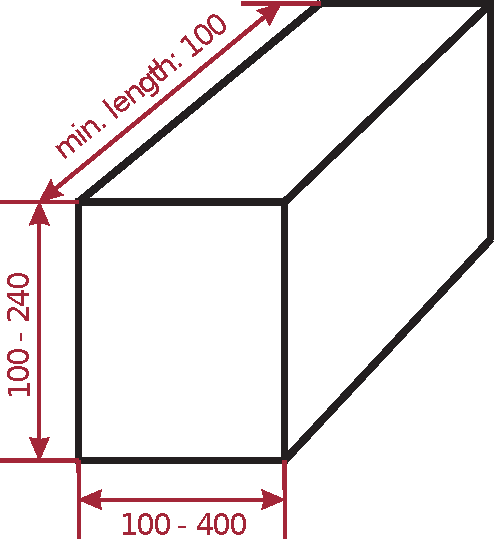
\includegraphics[height=.45\textheight]{../Material/Presentation/Obstacle.pdf}
        \end{column}
        \pause
        \begin{column}{.33\textwidth}
            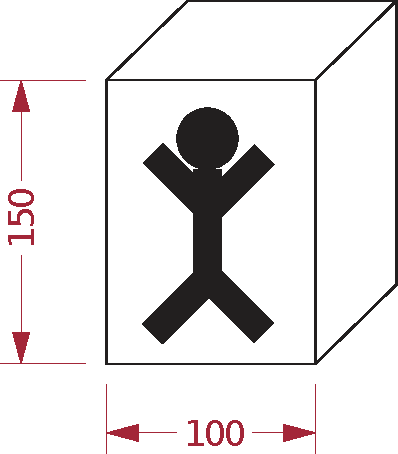
\includegraphics[height=.45\textheight]{../Material/Presentation/Pedestrian.pdf}
        \end{column}
        \pause
        \begin{column}{.33\textwidth}
            
\includegraphics[height=.45\textheight]{../Material/Presentation/Sign.pdf}
        \end{column}
    \end{columns}
    \pause
    \begin{itemize}
        \item Hindernisse und Fußgänger sind nicht anhand der Punktwolke unterscheidbar
            \pause
        \item Steigungen mit bis zu $10^\circ$
    \end{itemize}
\end{frame}

\begin{frame}
    \frametitle{Stand der Technik}
    \begin{itemize}
        \item Kombinierte Detektion und Klassifikation mit \acf{cnn}
            \pnote{Punktwolke oftmals als Voxel oder 2D-Karte repräsentiert}
            \pause
        \item Langsam ohne \ac{gpu} (Abschätzung: $30\si{\s}$ für Complex-YOLO)
            \pnote{Abschätzung auf Basis von YOLO auf Fahrzeug}
            \pause
        \item Schneller: Seperate Detektion und Klassifikation
            \pnote{Clustering mit ConnComp, Klassifikation mit K-NN, SVM, CNN}
            \pause
        \item Primär für Lidar Daten
            \pnote{Stereo PWs sind dichter aber mehr outlier}
            \pause
        \item Für Stereo: Oftmals auf Disparitätsbildern
            \pnote{Nachbarschaft nicht korrekt}
            \pause
        \item Nachbarschaft wird in Punktwolken besser repräsentiert \xfootcite{Wang19}
            \pnote{Standard Lidar Algorithmen auf Stereo PWs besser als SOTA für Disparitätsbilder}
    \end{itemize}
\end{frame}

\begin{frame}
    \frametitle{Algorithmus}
    \begin{itemize}
        \item Adaptierte Version von \cite{AttBen17}\xfootcite{AttBen17} für Stereodaten
            \pnote{Getrennte Pipeline, anpassungen für Stereo}
            \pause
        \item Vorgehen: 
            \pause
            \begin{itemize}
                \item Segmentierung
                    \pnote{Jedem Punkt eine Klasse zuordenen}
                    \pause
                \item Clustering
                    \pnote{Punkte gleicher Klasse zusammenfassen}
                    \pause
                \item Extraktion von Pseudotiefenbilder
                    \pnote{Klassifikation einfacher und schneller als auch PW}
                    \pause
                \item Klassifikation
                    \pnote{CNN}
                    \pause
            \end{itemize}
        \item Zusätzlich: Bounding-Box- und Bodenschätzung
            \pnote{Für spätere Plannung relevant}
    \end{itemize}
\end{frame}

\begin{frame}
    \frametitle{Algorithmus - Segmentierung}
    Klassen: Sparse, Ground, High-Foreground, Low-Foreground
    \begin{figure}
        \centering
        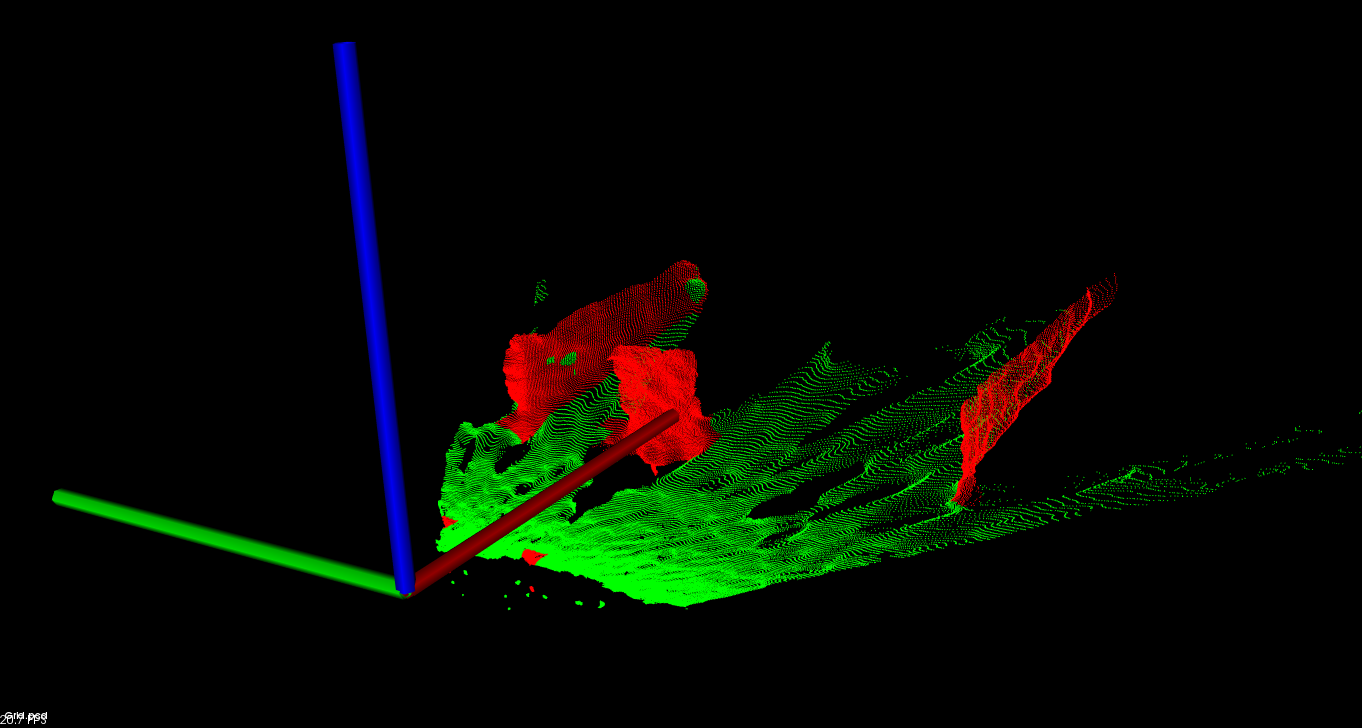
\includegraphics[width=\textwidth]{../Material/Presentation/grid.png}
    \end{figure}
    \pnote{Punktwolke in Zellen einordnen}
    \pnote{Wenn weniger als 8 Punkte dann Sparse}
    \pnote{Wenn Differenz Max-Min kleiner 0.25m dann Ground}
    \pnote{Wenn maximum 1.4m höher als Fahrzeug oder max-min > 3.1m dann HF}
    \pnote{Sonst LF}
\end{frame}

\begin{frame}
    \frametitle{Algorithmus - Clustering}
    \begin{figure}
        \centering
        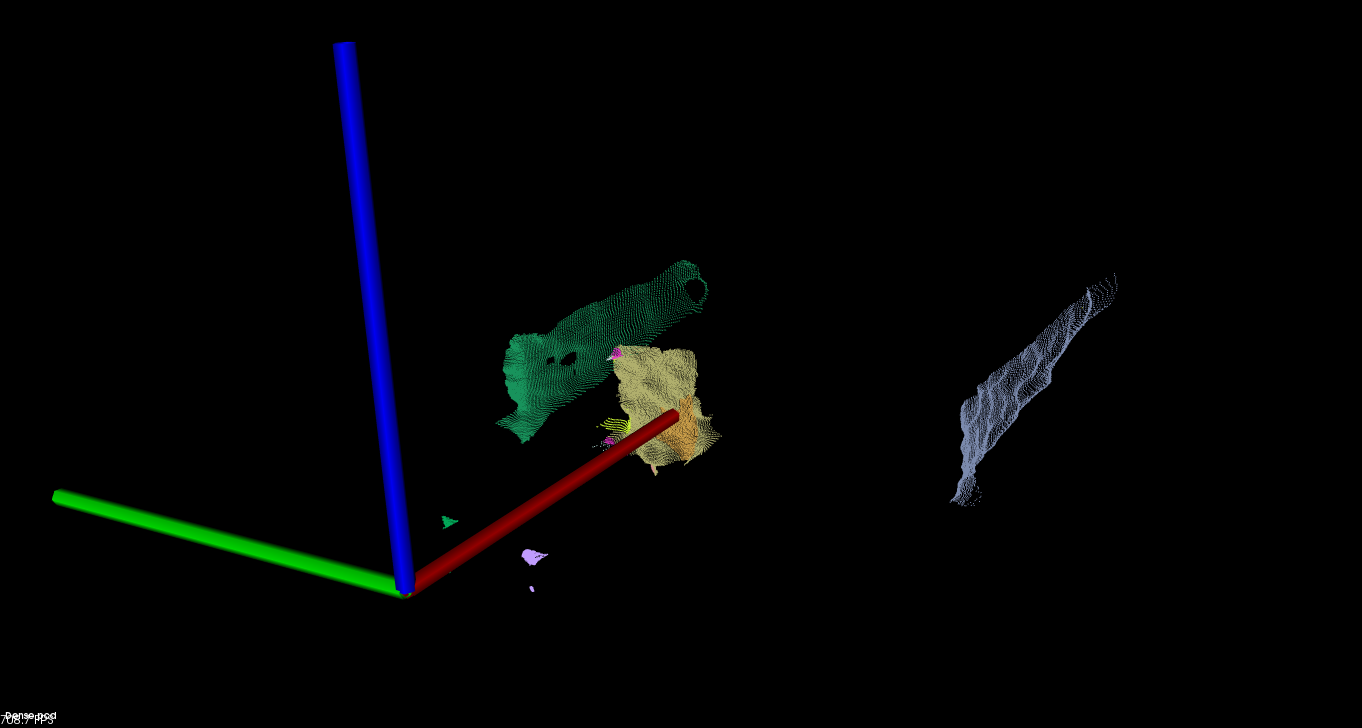
\includegraphics[width=\textwidth]{../Material/Presentation/objects.png}
    \end{figure}
    \pnote{Connecte Components auf zwei Ebenen}
    \pnote{Zuerst auf Zellen Ebene, mergen wenn Maximum-Differenz klein}
    \pnote{Dann jede Zelle in drei Subzellen teilen}
    \pnote{Cluster trennen wenn zu geringe Dichtedifferenz zwischen Subzellen}
\end{frame}

\begin{frame}
    \frametitle{Ausrichtung bestimmen}
    \begin{columns}
        \begin{column}{.5\textwidth}
            \begin{itemize}
                \item<1-> Hauptkomponenten-analyse des Clusters
                    \pnote{Richtungen mit größter Veränderung finden}
                \item<2-> Wichtigste nicht vertikale Hauptachse
                    \pnote{Für hohe Objekte, z.B. Fußgänger, ist erste HA quasi Vertikal}
                \item<3-> Für erste HA: Winkel zur $z$-Achse bestimmen
                    \pnote{Dadurch feststellen ob primär horizontal oder vertikal}
                \item<4-> Wenn größer als $45^\circ$ dann erste Hauptachse
                    \pnote{Entsprechende horizontale Komponente der HA nehmen}
            \end{itemize}
        \end{column}
        \begin{column}{.5\textwidth}
            \begin{figure}
                \centering
                \begin{tikzpicture}
                    \node[anchor=south west,inner sep=0] at (0,0) {
                        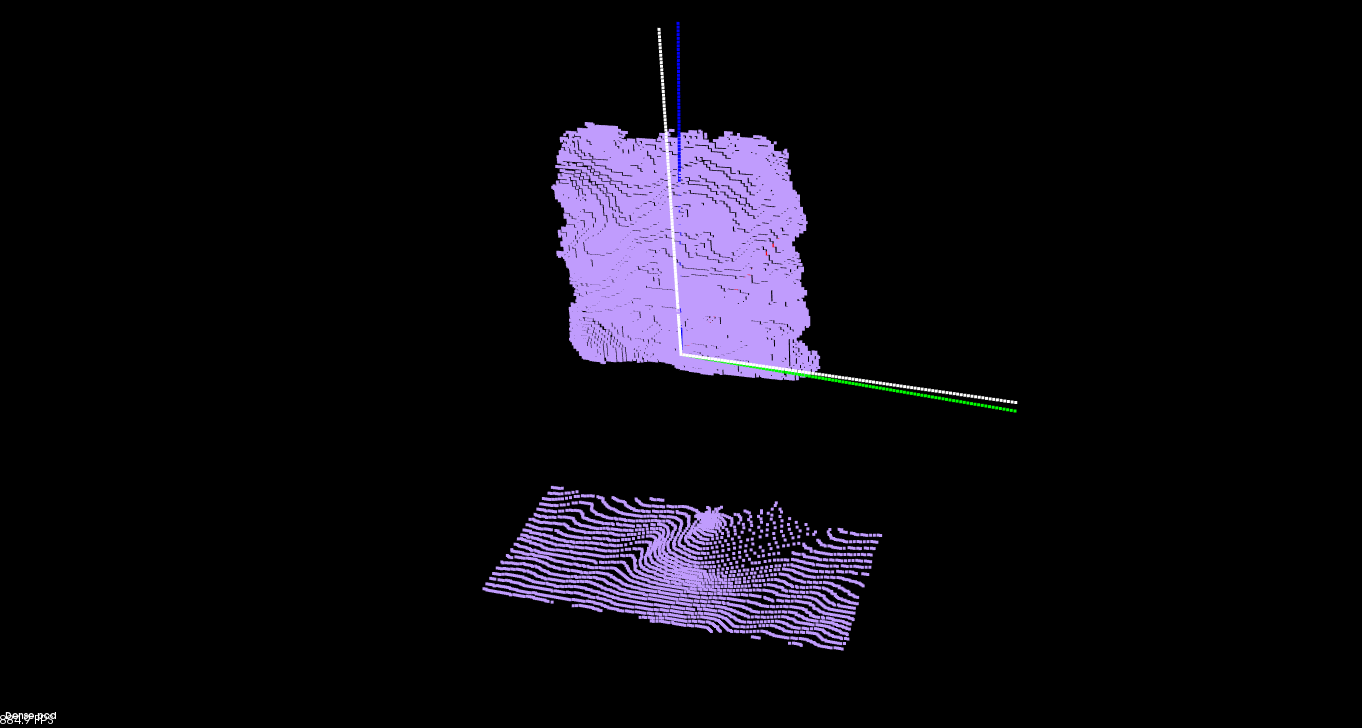
\includegraphics[width=\textwidth]{pca.png}
                    };
                    \coordinate (0) at (2.42,2.37);
                    \coordinate (y) at (2.27,4.43);
                    \coordinate (b) at (2.4,4.47);
                    \coordinate (g) at (4.52,2.0);
                    \coordinate (x) at (4.52,2.07);
                    
                    \draw[white,line width=0.6mm,->] (0) -- (y);
                    \draw[white,line width=0.6mm,->] (0) -- (x);
                    \draw[green,line width=0.6mm,->] (0) -- (g);
                    \draw[blue, line width=0.6mm,->] (0) -- (b);
                \end{tikzpicture}
            \end{figure}
        \end{column}
    \end{columns}
\end{frame}

\begin{frame}
    \frametitle{Algorithmus - Extraktion und Klassifikation}
    \pnote{Projektionsebene aus Heading und z-Achse}
    \pnote{Alle Punkte aus Projektionsebene projezieren, Helligkeit je nach Entfernung}
    \pnote{Größe 96x96}
    \begin{columns}
        \begin{column}{.5\textwidth}
            \begin{figure}
                \centering
                
\includegraphics[width=\textwidth]{../Material/Presentation/image_0.png}
                \caption{Hindernis}
            \end{figure}
        \end{column}
        \begin{column}{.5\textwidth}
            \begin{figure}
                \centering
                
\includegraphics[width=\textwidth]{../Material/Presentation/image_2.png}
                \caption{Schild}
            \end{figure}
        \end{column}
    \end{columns}
    \pause
    Klassifikation mit \ac{cnn}: Vehicle, Short Facade, Street Clutter, Pedestrian
    \pnote{4 Conv, Dense, Softmax}
\end{frame}

\begin{frame}
    \frametitle{Verbesserungen - Segmentierung}
    \begin{itemize}
        \item Low- und High-Foreground kombiniert
            \pnote{Carolo-Cup kennt nur kleine Objekte, Unterscheidung nicht relevant}
            \pause
        \item Klassifikation über minimum/maximum anfällig
            \pnote{Stereo PWs haben viele Outlier, minimum und maximum wird nur durch einen Punkt bestimmt}
            \pause
        \item Klassifikation über Varianz
            \pnote{Varianz robuster, beschreibt auch die Höhenverteilung}
    \end{itemize}
\end{frame}

\begin{frame}
    \frametitle{Verbesserungen - Extraktion und Klassifikation}
    \begin{itemize}
        \item Hauptkomponentenanalyse nicht notwendig
            \pnote{Boxen unabhängig von Betrachtungsrichtung}
            \pnote{Schilder am meisten Informationen von vorne}
            \pause
        \item Kleinere Pseudotiefenbilder
            \pnote{Alle Informationen in 40x40 Pixel}
            \pause
        \item Median-Filter für Distanzinvarianz
            \pnote{Um Löcher zu schließen}
            \pause
        \item Nur drei Klassen: Obstacle, Clutter, Pedestrian
            \pnote{Gibt keine Short Facade laut Regelwerk}
            \pause
        \item Kleineres \ac{cnn} ausreichend
            \pnote{Schneller, Input Kleiner, nur 2 Conv}
            \pause
        \item Trainingsdatensatz: 2406 Bilder
            \pnote{Training mit Data-Augmentation x10, Max-Pooling, Adadelta}
    \end{itemize}
\end{frame}

\begin{frame}
    \frametitle{Verbesserungen - Textur}
    \begin{itemize}
        \item Für Kitti/Lehr: Farbinformation für jeden Punkt
            \pnote{Da direkt von Farbkamera kommen information direkt vorhanden}
            \pause
        \item Wird statt Tiefeninformation genutzt
            \pnote{Dadurch komplexe Objekte gut zu unterscheiden}
            \pause
    \end{itemize}
    \begin{figure}[h!]
        \centering
        \begin{subfigure}[c]{0.3\textwidth}
            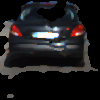
\includegraphics[width=\textwidth]{../Material/texture222_0.png}
        \end{subfigure}
        \begin{subfigure}[c]{0.3\textwidth}
            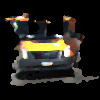
\includegraphics[width=\textwidth]{../Material/texture222_1.png}
        \end{subfigure}
        \begin{subfigure}[c]{0.3\textwidth}
            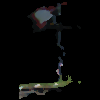
\includegraphics[width=\textwidth]{../Material/texture0_0.png}
        \end{subfigure}
    \end{figure}
\end{frame}

\begin{frame}
    \frametitle{Erweiterungen - Bounding Box}
    \begin{columns}
        \begin{column}{.5\textwidth}
            \begin{itemize}
                \item Zum Umfahren von Hindernissen/Fußgängern, bzw. Klassifikation von Schilder 
                    \pnote{In beiden Fällen ist groß nicht schlecht}
                \item<2-> Zuerst Ausrichtung bestimmen
                    \pnote{Verweis auf Hauptkomponentenanalyse}
                \item<3-> Dann Ausdehnung in $x$ und $y$ Richtung bestimmen
                    \pnote{Entlang der Hauptachse, z Ignorieren}
                \item<4-> Ausdehnung in $z$ Richtung bestimmen
                    \pnote{Hier keine Drehung, da alles flach}
            \end{itemize}
        \end{column}
        \begin{column}{.5\textwidth}
            \only<1>{
    \begin{figure}[h!]
        \centering
        \begin{tikzpicture}
            \fill[fill=primary] (4,4) circle (0.2cm);
            \fill[fill=primary] (4.5,4.5) circle (0.2cm);
            \fill[fill=primary] (5,5) circle (0.2cm);
            \fill[fill=primary] (5.5,5.5) circle (0.2cm);
            \fill[fill=primary] (6,6) circle (0.2cm);
            \fill[fill=primary] (4.5,5.5) circle (0.2cm);
            \fill[fill=primary] (5.5,4.5) circle (0.2cm);
            \fill[fill=primary] (4,5) circle (0.2cm);
            \fill[fill=primary] (6,5) circle (0.2cm);
            \fill[fill=primary] (5,4) circle (0.2cm);
            \fill[fill=primary] (5,6) circle (0.2cm);

            \node at(3,3) (){};
            \node at(7.5,7.5) (){};
        \end{tikzpicture}
    \end{figure}
}
\only<2>{
    \begin{figure}[h!]
        \centering
        \begin{tikzpicture}
            \fill[fill=primary] (4,4) circle (0.2cm);
            \fill[fill=primary] (4.5,4.5) circle (0.2cm);
            \fill[fill=primary] (5,5) circle (0.2cm);
            \fill[fill=primary] (5.5,5.5) circle (0.2cm);
            \fill[fill=primary] (6,6) circle (0.2cm);
            \fill[fill=primary] (4.5,5.5) circle (0.2cm);
            \fill[fill=primary] (5.5,4.5) circle (0.2cm);
            \fill[fill=primary] (4,5) circle (0.2cm);
            \fill[fill=primary] (6,5) circle (0.2cm);
            \fill[fill=primary] (5,4) circle (0.2cm);
            \fill[fill=primary] (5,6) circle (0.2cm);

            \draw[line width=2pt,->] (5,5) -- (7,7);

            \node at(3,3) (){};
            \node at(7.5,7.5) (){};
        \end{tikzpicture}
    \end{figure}
}
\only<3->{
    \begin{figure}[h!]
        \centering
        \begin{tikzpicture}
            \fill[fill=primary] (4,4) circle (0.2cm);
            \fill[fill=primary] (4.5,4.5) circle (0.2cm);
            \fill[fill=primary] (5,5) circle (0.2cm);
            \fill[fill=primary] (5.5,5.5) circle (0.2cm);
            \fill[fill=primary] (6,6) circle (0.2cm);
            \fill[fill=primary] (4.5,5.5) circle (0.2cm);
            \fill[fill=primary] (5.5,4.5) circle (0.2cm);
            \fill[fill=primary] (4,5) circle (0.2cm);
            \fill[fill=primary] (6,5) circle (0.2cm);
            \fill[fill=primary] (5,4) circle (0.2cm);
            \fill[fill=primary] (5,6) circle (0.2cm);

            \draw[line width=2pt,->] (5,5) -- (7,7);
            \coordinate (a) at (4.5, 3.2);
            \coordinate (b) at (6.8, 5.5);
            \coordinate (c) at (5.5, 6.8);
            \coordinate (d) at (3.2, 4.5);
            \draw[line width=2pt] (a) -- (b);
            \draw[line width=2pt] (b) -- (c);
            \draw[line width=2pt] (c) -- (d);
            \draw[line width=2pt] (d) -- (a);

            \node at(3,3) (){};
            \node at(7.5,7.5) (){};
        \end{tikzpicture}
    \end{figure}
}

        \end{column}
    \end{columns}
\end{frame}

\begin{frame}
    \frametitle{Erweiterungen - Bodenschätzung}
    \begin{columns}
        \begin{column}{.5\textwidth}
            \begin{itemize}
                \item Alle Ground-Zellen werden Berücksichtigt
                    \pnote{Verweis Segmentierung}
                \item<2-> Mittel der $z$-Werte pro Zelle
                    \pnote{Mittlere Höhe in Zelle}
                \item<3-> Pro Zelle ein Punkt
                    \pnote{In mitte der Zelle mit Mittelwert $z$ als Höhe}
                \item<4-> Ebene mit Methode der kleinsten Quadrate
                    \pnote{Nur eine Ebene, am Anfang von Steigungen kann problematisch}
            \end{itemize}
        \end{column}
        \begin{column}{.5\textwidth}
            \only<1>{
\begin{tikzpicture}[scale=0.4]
    \fill[fill=gray] (0,-0.2) circle (0.2cm);
    \fill[fill=gray] (1,0.1) circle (0.2cm);
    \fill[fill=gray] (2,0.6) circle (0.2cm);
    \fill[fill=gray] (3,0.85) circle (0.2cm);
    \fill[fill=gray] (4,1.15) circle (0.2cm);
    \fill[fill=gray] (5,1.2) circle (0.2cm);
    \fill[fill=gray] (6,1.4) circle (0.2cm);
    \fill[fill=gray] (7,1.9) circle (0.2cm);
    \fill[fill=gray] (8,2.1) circle (0.2cm);
    \fill[fill=gray] (9,2.3) circle (0.2cm);
    \fill[fill=gray] (10,2.6) circle (0.2cm);
    \fill[fill=gray] (11,2.7) circle (0.2cm);

    \fill[fill=gray] (6,2.4) circle (0.2cm);
    \fill[fill=gray] (7,2.9) circle (0.2cm);
    \fill[fill=gray] (8,3.1) circle (0.2cm);
    \fill[fill=gray] (6,3.4) circle (0.2cm);
    \fill[fill=gray] (7,3.9) circle (0.2cm);
    \fill[fill=gray] (8,4.1) circle (0.2cm);

    \node at(-1,-0.25) (){};
    \node at(12,5) (){};
\end{tikzpicture}
}
\only<2>{
\begin{tikzpicture}[scale=0.4]
    \fill[fill=gray] (0,-0.2) circle (0.2cm);
    \fill[fill=gray] (1,0.1) circle (0.2cm);
    \fill[fill=gray] (2,0.6) circle (0.2cm);
    \fill[fill=gray] (3,0.85) circle (0.2cm);
    \fill[fill=gray] (4,1.15) circle (0.2cm);
    \fill[fill=gray] (5,1.2) circle (0.2cm);
    \fill[fill=gray] (6,1.4) circle (0.2cm);
    \fill[fill=gray] (7,1.9) circle (0.2cm);
    \fill[fill=gray] (8,2.1) circle (0.2cm);
    \fill[fill=gray] (9,2.3) circle (0.2cm);
    \fill[fill=gray] (10,2.6) circle (0.2cm);
    \fill[fill=gray] (11,2.7) circle (0.2cm);

    \fill[fill=gray] (6,2.4) circle (0.2cm);
    \fill[fill=gray] (7,2.9) circle (0.2cm);
    \fill[fill=gray] (8,3.1) circle (0.2cm);
    \fill[fill=gray] (6,3.4) circle (0.2cm);
    \fill[fill=gray] (7,3.9) circle (0.2cm);
    \fill[fill=gray] (8,4.1) circle (0.2cm);

    \draw[dashed, line width=0.3mm] (2.5,-0.5) -- (2.5,5);
    \draw[dashed, line width=0.3mm] (5.5,-0.5) -- (5.5,5);
    \draw[dashed, line width=0.3mm] (8.5,-0.5) -- (8.5,5);

    \node at(-1,-0.25) (){};
    \node at(12,5) (){};
\end{tikzpicture}
}
\only<3>{
\begin{tikzpicture}[scale=0.4]
    \fill[fill=gray] (0,-0.2) circle (0.2cm);
    \fill[fill=gray] (1,0.1) circle (0.2cm);
    \fill[fill=gray] (2,0.6) circle (0.2cm);
    \fill[fill=gray] (3,0.85) circle (0.2cm);
    \fill[fill=gray] (4,1.15) circle (0.2cm);
    \fill[fill=gray] (5,1.2) circle (0.2cm);
    \fill[fill=gray] (6,1.4) circle (0.2cm);
    \fill[fill=gray] (7,1.9) circle (0.2cm);
    \fill[fill=gray] (8,2.1) circle (0.2cm);
    \fill[fill=gray] (9,2.3) circle (0.2cm);
    \fill[fill=gray] (10,2.6) circle (0.2cm);
    \fill[fill=gray] (11,2.7) circle (0.2cm);

    \fill[fill=gray] (6,2.4) circle (0.2cm);
    \fill[fill=gray] (7,2.9) circle (0.2cm);
    \fill[fill=gray] (8,3.1) circle (0.2cm);
    \fill[fill=gray] (6,3.4) circle (0.2cm);
    \fill[fill=gray] (7,3.9) circle (0.2cm);
    \fill[fill=gray] (8,4.1) circle (0.2cm);

    \draw[dashed, line width=0.3mm] (2.5,-0.5) -- (2.5,5);
    \draw[dashed, line width=0.3mm] (5.5,-0.5) -- (5.5,5);
    \draw[dashed, line width=0.3mm] (8.5,-0.5) -- (8.5,5);

    \fill[fill=primary] (1,0.17) circle (0.2cm);
    \fill[fill=primary] (4,1.07) circle (0.2cm);
    \fill[fill=primary] (10,2.5) circle (0.2cm);

    \node at(-1,-0.25) (){};
    \node at(12,5) (){};
\end{tikzpicture}
}
\only<4>{
\begin{tikzpicture}[scale=0.4]
    \fill[fill=gray] (0,-0.2) circle (0.2cm);
    \fill[fill=gray] (1,0.1) circle (0.2cm);
    \fill[fill=gray] (2,0.6) circle (0.2cm);
    \fill[fill=gray] (3,0.85) circle (0.2cm);
    \fill[fill=gray] (4,1.15) circle (0.2cm);
    \fill[fill=gray] (5,1.2) circle (0.2cm);
    \fill[fill=gray] (6,1.4) circle (0.2cm);
    \fill[fill=gray] (7,1.9) circle (0.2cm);
    \fill[fill=gray] (8,2.1) circle (0.2cm);
    \fill[fill=gray] (9,2.3) circle (0.2cm);
    \fill[fill=gray] (10,2.6) circle (0.2cm);
    \fill[fill=gray] (11,2.7) circle (0.2cm);

    \fill[fill=gray] (6,2.4) circle (0.2cm);
    \fill[fill=gray] (7,2.9) circle (0.2cm);
    \fill[fill=gray] (8,3.1) circle (0.2cm);
    \fill[fill=gray] (6,3.4) circle (0.2cm);
    \fill[fill=gray] (7,3.9) circle (0.2cm);
    \fill[fill=gray] (8,4.1) circle (0.2cm);

    \draw[dashed, line width=0.3mm] (2.5,-0.5) -- (2.5,5);
    \draw[dashed, line width=0.3mm] (5.5,-0.5) -- (5.5,5);
    \draw[dashed, line width=0.3mm] (8.5,-0.5) -- (8.5,5);

    \fill[fill=primary] (1,0.17) circle (0.2cm);
    \fill[fill=primary] (4,1.07) circle (0.2cm);
    \fill[fill=primary] (10,2.5) circle (0.2cm);

    \draw[line width=0.5mm] (-1,-0.25) -- (12,3);

    \node at(-1,-0.25) (){};
    \node at(12,5) (){};
\end{tikzpicture}
}

        \end{column}
    \end{columns}
\end{frame}

    \chapter{Evaluation} \label{sec:eval}
In the following chapter the performance of the algorithm is evaluated. 
The first section is a quantitative evaluation of the different steps of the pipeline and the end-to-end detection performance. The second
section evaluates the performance and highlights the strengths and weaknesses of the detection. In the third section
the computational performance, that is primarily the required time for the different steps, gets evaluated. In the next section the performance on
real world data is evaluated. Two different datasets are chosen: first the data acquired by a stereo camera in Ulm-Lehr as part of the MEC-View-Project \cite{mec} and second data from the Kitti dataset \cite{Menze2015CVPR}.  
Lastly the runtime of the algorithm is compared with other state of the art algorithms.

\section{Quantitative Evaluation}
To evaluate the performance of the algorithm 20 point clouds recorded on the vehicle with the \ac{d435} have been labeled by hand, in total there are 47 objects of interest in these point clouds. The point clouds show 22 obstacles and pedestrians and 25 signs. Ten of the 20 point clouds are recorded on the slope or show parts of the slope.
In each point cloud every point has been assigned one of the following classes:
\begin{itemize}
    \item Ground
    \item Sign
    \item Obstacle/Pedestrian
    \item Street Furniture
    \item Clutter
\end{itemize}
Obstacles and pedestrian are combined in one class as it is not possible to discriminate between them solely from the point cloud. 
The class "Clutter" represents all points that are outliers and thus do not belong to any class, Figure \ref{fig:eval:typeSparse} shows an example for such outlier points.
In contrast the class "Street Furniture" represents all points which are valid but do not belong to objects which are of interest, these objects include
things such as guardrails and walls.

\subsection{Segmentation}
The segmentation is the first step of the detection pipeline. In this step every cell gets a type assigned. The type gets decided based on the variance of the height of the points in each cell.

The performance gets evaluated in two ways, first on a per point level, that means the class of every point is compared with the actual class.
The second way is the evaluation on a per cell level, that means every cell is compared with the class of the cell. The ground truth class of the cells is
determined by the class with the largest number of points in the cell. If a cell contains less than eight points it is classified as Sparse, this is identical to how it is done in the algorithm.

To be able to not only see the correct detection rate but also the failure modes the data is shown in a confusion matrix. The rows represent predictions, that is the output of the algorithm, the columns the actual type of the point or cell.
The matrix consists of the points of all 20 ground truth point clouds.

The types of the labeled points are not the same as the types of the points after segmentation. To compare the points, the types of the ground truth data get mapped on the segmentation types.
The mapping is as follows: Sign and Obstacle/Pedestrian get mapped to the type Foreground, Clutter gets mapped to Sparse. The type Street Furniture is ignored, as the type corresponds to 
different types which are not of interest.

\begin{table}[h!]
    \centering
    \begin{tabular}{c|rrrrrr}
        \toprule
        \diagbox{Predicted}{Actual} & \multicolumn{2}{c}{Ground} & \multicolumn{2}{c}{Foreground} & \multicolumn{2}{c}{Sparse} \\
        \midrule
        Ground & 958,704 & (92.1\%) & 3,436 & (2.0\%) & 12,224 & (53.3\%) \\ 
        Foreground & 70,293 & (6.8\%) & 164,209 & (97.9\%) & 10,416 & (45.4\%)  \\ 
        Sparse & 11,688 & (1.1\%) & 71 & (0.04\%) & 273 & (1.2\%) \\ 
        \midrule
        Total & 1,040,685 && 167,716 && 22,913 \\
        \bottomrule
    \end{tabular}
    \caption{Confusion matrix on per point level}
    \label{tab:eval:confPoint}
\end{table}

The confusion matrix on point level (Table \ref{tab:eval:confPoint}) shows
that for the classes Ground and Foreground most points get
classified correctly.
The precision for ground points is 92\%, for the points labeled as Foreground the precision is 98\%. 
For the points classified as Sparse only a small number of the points is actually labeled as Sparse.
This is due to the fact, that many points which are labeled as Sparse
are actually in a cell with relevant points and thus are classified as
this class. An example for this problem can be seen in Figure \ref{fig:eval:typeSparse}

\begin{figure}[h!]
    \centering
    \begin{tikzpicture}
        \node[anchor=south west,inner sep=0] at (0,0) {
            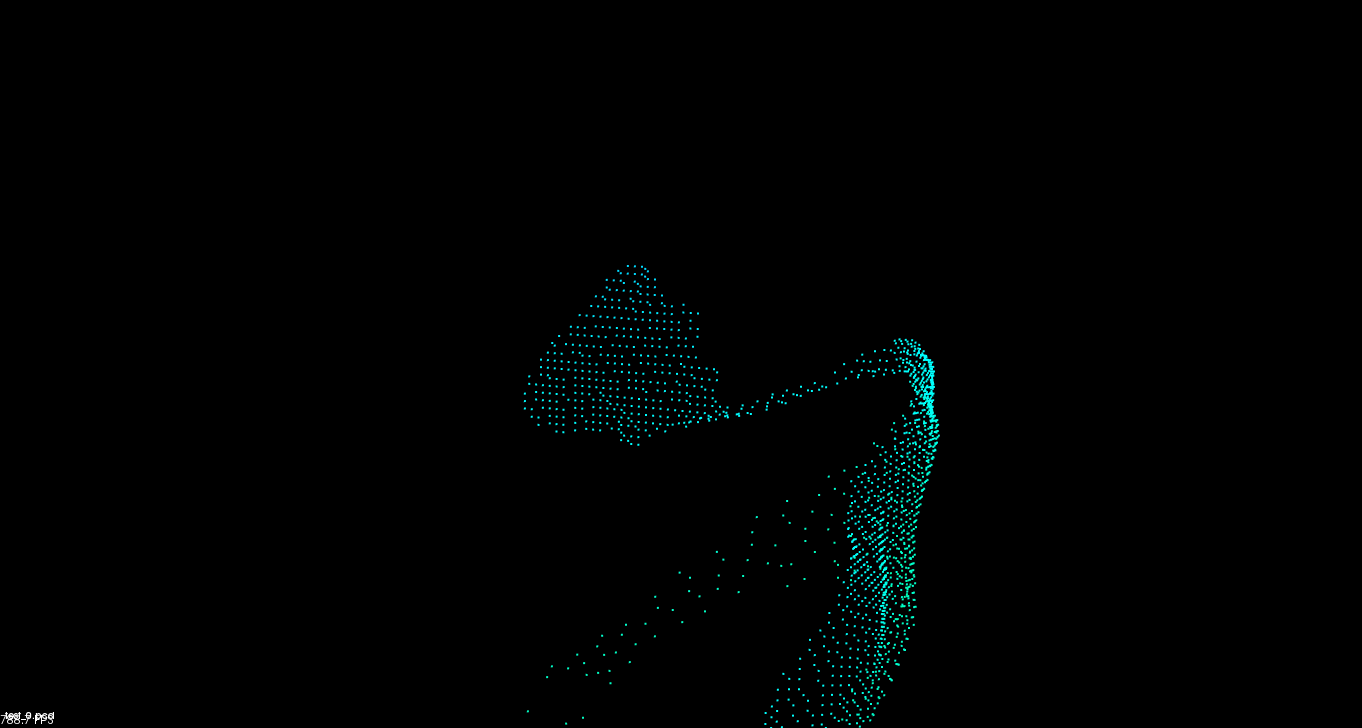
\includegraphics[width=\textwidth]{typeSparse.png}
        };
        \draw[draw=green, line width=0.1cm] (5.6,3.3) -- (8.3,3.3) -- (7.1,5.4) -- (5.6,3.3);
        \node at (5.5,4.5) {Sign};
        \draw[draw=red, line width=0.1cm] (9.2,4) ellipse (1.2 and 0.7);
        \node at (9.2,5.2) {Outlier};
    \end{tikzpicture}
    \caption{Outlier points next to a sign}
    \label{fig:eval:typeSparse}
\end{figure}

\begin{table}[h!]
    \centering
    \begin{tabular}{c|rrrrrr}
        \toprule
        \diagbox{Predicted}{Actual} & \multicolumn{2}{c}{Ground} & \multicolumn{2}{c}{Foreground} & \multicolumn{2}{c}{Sparse} \\
        \midrule
        Ground & 8,302 & (96.9\%) & 45 & (14.8\%) & 227 & (0.45\%) \\
        Foreground & 184 & (2.1\%) & 248 & (81\%) & 45 & (0.1\%) \\
        Sparse & 79 & (0.92\%) & 12 & (4.0\%) & 49,943 & (99.5\%) \\
        \midrule
        Total & 8,565 && 305 && 50,215 \\
        \bottomrule
    \end{tabular}
    \caption{Confusion matrix on cell level}
    \label{tab:eval:confCell}
\end{table}

For the classification on a per cell basis, the confusion matrix is shown in Table \ref{tab:eval:confCell}. 
The large number sparse cells in comparison to the number of sparse points is due to cells which do not contain any points, thus they are sparse but no points labeled sparse exist.
For all classes the majority of cells get labeled correctly. 
The precision for the ground cells is 97\%, for the classes labeled as Foreground the precision is 81\%, for the sparse cells the precision is 99\%.
The comparably high number of ground cells which have been labeled as Foreground is due to the outlier points (see Figures \ref{fig:eval:typeSparse} and \ref{sec:eval:outlier}).

When comparing the confusion matrices it can be seen that the precision on cell level is on average higher than those on the per point level. This is due to the non-uniformity of the cells, i.e. there are points of different classes in a single cell.

It can be concluded that the proposed heuristic yields a good precision for all classes. 
Especially the high precision for foreground points ($98\%$) provide a good basis for the object detection and clustering.

\subsection{Clustering and Bounding Box Estimation} \label{sec:eval:iou}
To assess the performance the \ac{iou} is calculated. 
This statistic measures the similarity of two sets by dividing the size of the intersection of both sets through the size of the union of both sets. 
For the bounding boxes the \ac{iou} is determined by the respective volumes.

The ground truth data is generated from the hand-labeled point clouds. Only objects which either belong to the class Sign or the class Obstacle/Pedestrian are considered for the evaluation.
For every object the bounding box is calculated identically to the real detection: the orientation of the box is estimated using the \ac{pca} of all points. The dimensions and
position are chosen such that all points of the cluster are in the bounding box.

The algorithm clusters all objects which belong to the class Foreground, as a result there are more bounding boxes in the detection than there are in the ground truth data.
For the evaluation only the relevant objects, that are the objects with the largest \ac{iou} relative to the ground truth, are used.

\begin{figure}[h!]
    \centering
    \begin{subfigure}[c]{0.75\textwidth}
        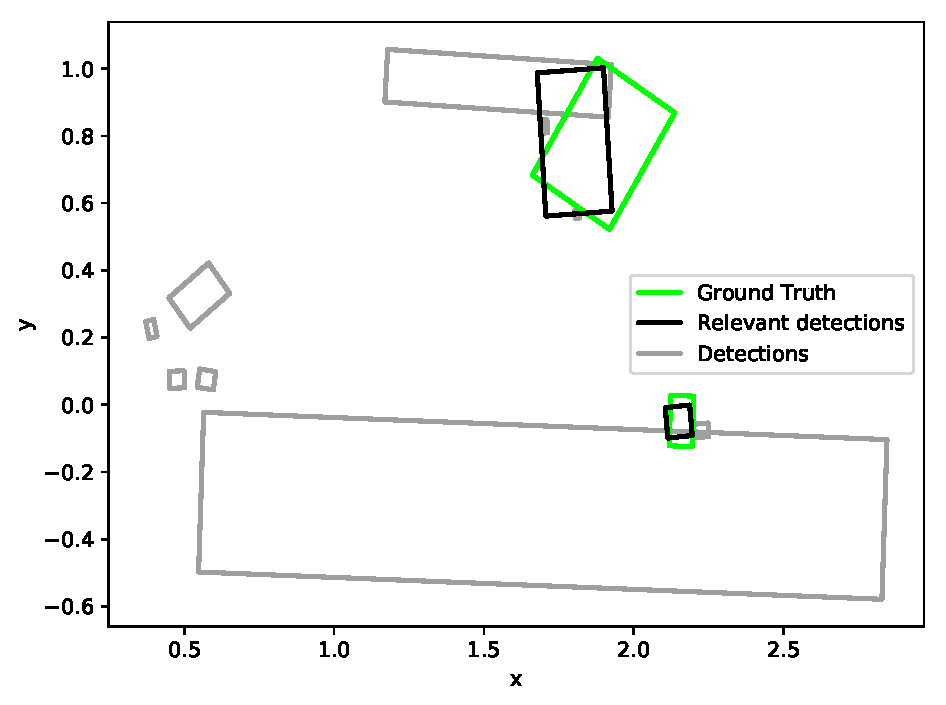
\includegraphics[width=\textwidth]{../Material/iou0.pdf}
        \subcaption{}
        \label{fig:eval:iou:0}
    \end{subfigure}

    \begin{subfigure}[c]{0.75\textwidth}
        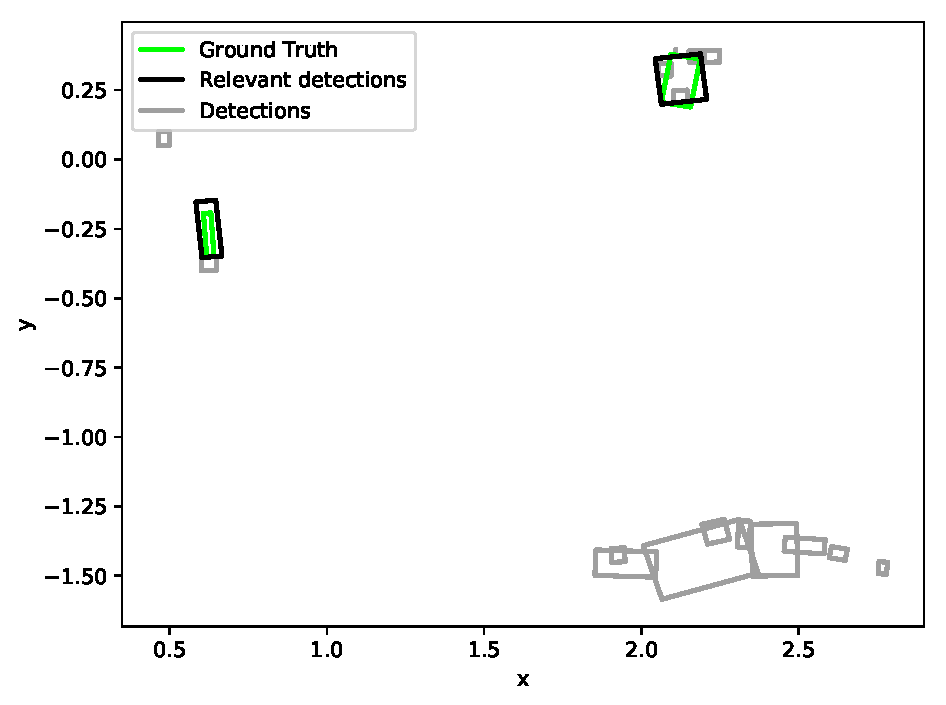
\includegraphics[width=\textwidth]{../Material/iou2.pdf}
        \subcaption{}
        \label{fig:eval:iou:2}
    \end{subfigure}
    \caption{Comparison of the estimated bounding boxes and the ground truth data, seen from above.}
    \label{fig:eval:iou}
\end{figure}

The \ac{iou} is calculated in 2D and 3D. For the 2D case the z-Axis is ignored and the \ac{iou} is only calculated by area as it can be seen in Figure \ref{fig:eval:iou}.
This information is the relevant information for the later stages of planning which are done solely in 2D. To evaluate the true performance the 3D bounding boxes are evaluated as well,
for this step the \ac{iou} is calculated based on the respective volumes.

Both \ac{iou}-scores are calculated for all 47 objects in the 20 ground truth point clouds. 
The average \ac{iou} for both cases can be seen in Table \ref{tab:eval:iou}.
The histogram of the respective values can be seen in Figure \ref{fig:eval:iouDist}.

\begin{table}[h!]
    \centering
    \begin{tabular}{cc}
        \toprule
        Average 2D & 0.444 \\
        Average 3D & 0.321 \\
        \bottomrule
    \end{tabular}
    \caption{Average IoU Scores} 
    \label{tab:eval:iou}
\end{table}

\begin{figure}[h!]
    \centering
    \begin{subfigure}[c]{0.49\textwidth}
        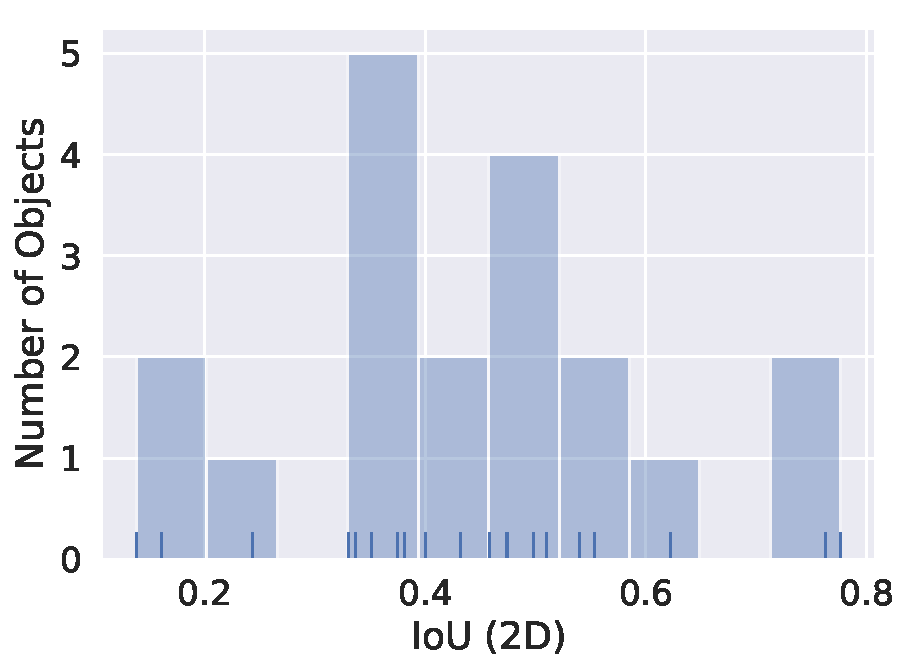
\includegraphics[width=\textwidth]{../Material/iouDist2.pdf}
        \subcaption{2D}
    \end{subfigure}
    \begin{subfigure}[c]{0.49\textwidth}
        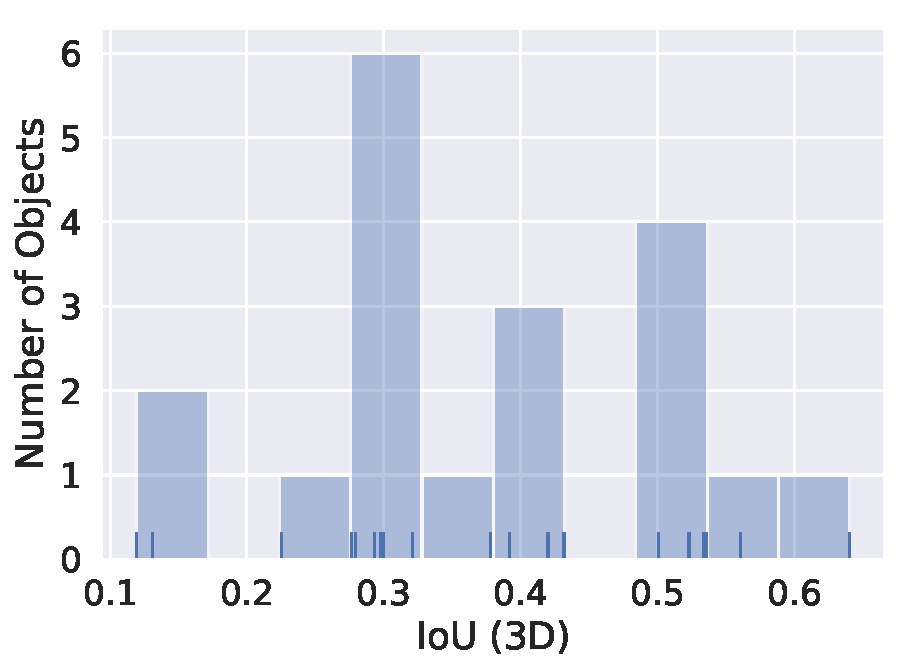
\includegraphics[width=\textwidth]{../Material/iouDist3.pdf}
        \subcaption{3D}
    \end{subfigure}
    \caption{Distribution of the IoU-Scores}
    \label{fig:eval:iouDist}
\end{figure}

The \ac{iou}-Scores are quite low when compared to typical values for computer-vision tasks, this is due to the two major differences: first the heading for the bounding box is not fixed, as a result the bounding boxes can be rotated relative to each other, this can be seen for the upper bounding box in Figure \ref{fig:eval:iou:0}, which only yields an 2D-\ac{iou} of 0.42.
The second difference is the third dimension, which leads to a smaller \ac{iou} as well.

It is clearly visible that the histogram for the three dimensional \ac{iou} is shifted to the left when compared with the one for the two dimensional case. This shows that the values for the 3D case are in general lower than the values for the 2D case.

Figure \ref{fig:eval:iou} shows that for most objects the bounding box is larger than ground truth bounding box. Thus obstacles can be passed reliably without touching them, as the minimum distance between obstacles is $1\si{\m}$ \cite{Carolo-CupRegelwerk} the large bounding box is not an issue. For signs a large bounding box results in a large region of interest, this simplifies the classification as the complete sign is inside the bounding box.

\subsection{Classification}
For every cluster an image is extracted and used for classification. The classification is done with a \ac{cnn}.

Every image is assigned one of three classes: Sign, Obstacle or Clutter. 
The class Obstacle includes pedestrians as well.

For evaluation a separate dataset which has not been used for training has been labeled.
It consists of 657 patches extracted from the 20 ground truth point clouds.
Of all patches 37 patches show objects of interest, that is obstacles and signs,
which have been detected by the algorithm. The number of patches is lower than the number of objects, this is because the algorithm is not able to detect every object correctly.

\begin{table}[h!]
    \centering
    \begin{tabular}{c|rrrrrr}
        \toprule
        \diagbox{Predicted}{Actual} & \multicolumn{2}{c}{Clutter} & \multicolumn{2}{c}{Obstacle} & \multicolumn{2}{c}{Sign} \\
        \midrule
        Clutter & 555 & (89.5\%) & 3 & (15.8\%) & 3 & (16.7\%) \\
        Obstacle & 49 & (7.9\%) & 15 & (78.9\%) & 1 & (5.6\%) \\
        Sign & 16 & (2.5\%) & 1 & (5.2\%) & 14 & (77.8\%) \\
        \midrule
        Total & 620 && 19 && 18 \\
        \bottomrule
    \end{tabular}
    \caption{Confusion matrix for the classification}
    \label{tab:eval:class}
\end{table}

Most of the relevant objects are classified correctly. The majority of patches that have been classified
wrong are Clutter which are either classified as Obstacles or Signs. 

By looking at the classification as a binary classification problem, that is by combining the classes Obstacle and Sign into one class "relevant" a second confusion matrix can be created, this can be seen in Table \ref{tab:eval:classBin}. 
Furthermore the precision, recall and $F_1$-score can be calculated \cite{informationRetrieval}. 
The recall is the number of correctly labeled patches divided by the total number of patches for this class. 
The $F_1$-score is the harmonic mean of precision and recall.
The results can be seen in Equation \ref{eqn:eval:classPrecision}.

\begin{table}[h!]
    \centering
    \begin{tabular}{c|rrrr}
        \toprule
        \diagbox{Predicted}{Actual} & \multicolumn{2}{c}{Relevant} & \multicolumn{2}{c}{Clutter} \\
        \midrule
        Relevant & 31 & (83.8\%) & 65 & (10.5\%) \\
        Clutter & 6 & (16.2\%) & 555 & (89.5\%) \\
        \midrule
        Total & 37 && 620 \\
        \bottomrule
    \end{tabular}
    \caption{Evaluation of the classification as binary classification problem}
    \label{tab:eval:classBin}
\end{table}

%https://medium.com/@jonathan_hui/map-mean-average-precision-for-object-detection-45c121a31173
\begin{eqnarray}
    \label{eqn:eval:classPrecision}
    \text{Precision} &=& \frac{31}{31 + 65} = 0.32\\
    \text{Recall} &=& \frac{31}{31+6} = 0.84 \\
    F_1 &=& 2 \cdot \frac{0.84 \cdot 0.32}{0.84+ 0.32} = 0.46
\end{eqnarray}

It is more important to detect all relevant objects than to achieve a high precision, thus the classification has been tuned to produce a high recall rate (84\%). The high number of false positives which result in a low precision can be tolerated because according to the Carolo-Cup rules \cite{Carolo-CupRegelwerk} there are no objects other than obstacles or signs on the road.

\subsection{Overall Performance}
The presented algorithm is an end-to-end approach for object detection in point clouds, thus the overall performance is evaluated.

The performance is evaluated similar to \cite{AttBen17}: for every object category the precision, recall and $F_1$-score is calculated. For the evaluation the detected object is compared with the object with the largest \ac{iou} in the ground truth data.

\begin{table}[h!]
    \centering
    \begin{tabular}{c|c|rrr}
        \toprule
        Category & Number of Objects & Pr & Rc & $F_1$\\
        \midrule
        Obstacle/Pedestrian & 20 & 100\% & 84\% & 91\% \\
        Sign & 18 & 78\% & 100\% & 88\% \\
        \midrule
        Average/Sum & 38 & 89\% & 92\% & 90\% \\
        \bottomrule
    \end{tabular}
    \caption{Overall performance of the proposed algorithm. Notations: Precision (Pr), Recall (Rc), $F_1$-score ($F_1$).}
    \label{tab:eval:overallProposed}
\end{table}

\begin{table}[h!]
    \centering
    \begin{tabular}{c|c|rrr}
        \toprule
        Category & Number of Objects & Pr & Rc & $F_1$\\
        \midrule
        Obstacle/Pedestrian & 20 & 100\% & 80\% & 89\% \\
        Sign & 17 & 71\% & 100\% & 83\% \\
        \midrule
        Average/Sum & 37 & 86\% & 90\% & 86\% \\
        \bottomrule
    \end{tabular}
    \caption{Overall performance of \cite{AttBen17}. Notations: Precision (Pr), Recall (Rc), $F_1$-score ($F_1$).}
    \label{tab:eval:overallBnb}
\end{table}

The performance of the proposed algorithm is shown in Table \ref{tab:eval:overallProposed} compared with the algorithm presented in \cite{AttBen17} which is shown in Table \ref{tab:eval:overallBnb}. 
Of the 47 objects in the 20 ground truth point clouds the proposed algorithm detects 38, the other algorithm detects only 37 objects. This yields an detection rate of 81\% and 79\% respectively.

For the average $F_1$-score the proposed algorithm is also superior to the detection presented in \cite{AttBen17}, with 90\% and 86\% respectively. On Lidar data \cite{AttBen17} achieves similar results, with a precision of 86\%, a recall of 83\% and a $F_1$-score of 85\%, albeit with four instead of three classes.

It should be taken into consideration that the dataset used for evaluation consists of less point clouds than the one used by \cite{AttBen17}.
Nonetheless the improvements of the algorithm result in a 2 percentage point higher detection rate, the precision is improved by 3 percentage points, the recall by 2 percentage points and the $F_1$-score by 4 percentage points.

\subsection{Ground Estimate}
For the evaluation all points of the 20 ground truth point clouds which are assigned the label ground are taken into account.
For each of these points the distance to the approximated plane is calculated.
Over all point clouds there are $1,691,693$ points which are part of the ground.

\begin{figure}[h!]
    \centering
    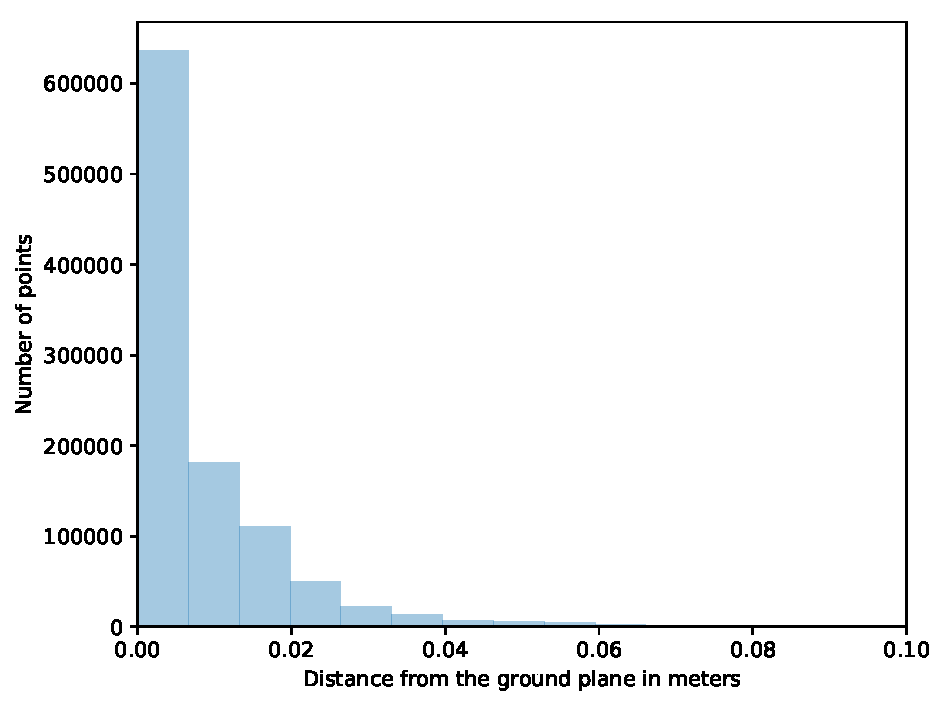
\includegraphics[width=\textwidth]{../Material/ground.pdf}
    \caption{Distribution of the distance to the plane}
    \label{fig:eval:groundDist}
\end{figure}

Figure \ref{fig:eval:groundDist} shows the distribution of the distances to the ground plane. 
It can be seen that most points are close to the estimated plane. Over all points the average absolute distance to the plane is 9.3 millimeters. The maximum error is 33cm, the point which yields this error is approximately $2\si{\m}$ from the vehicle after a slope on a flat part of the track, the estimated plane approximates the slope and not the flat part.

For situations in which the ground can not be approximated by a single plane the estimate yields the expected error. The plane has a slope, but the slope is smaller than the slope of the actual ground.
In situations in which the ground can be approximated by a single plane the error is small, in the ground truth data $71\%$ of all points are closer than $1\si{\cm}$ to the estimated plane. Thus the slope can be detected using the ground plane estimate. 

\subsection{Comparison with the current obstacle detection}
The proposed algorithm is intended to replace the obstacle detection currently used on the vehicle (see \ref{sec:det:obstDet}), thus the performance of the algorithms should be compared.
For the comparison the \ac{iou} scores are used, as described in section \ref{sec:eval:iou}.
The \ac{iou} is calculated in two ways: once only for the detected objects and second for all existing objects, objects that are not detected yield an \ac{iou} of $0$ for this score.

As the obstacle detection is intended to only detect obstacles, only clusters labeled as obstacles are taken into account. Over the 20 ground truth point clouds there are 22 objects labeled as obstacles. For the evaluation only the 2D-\ac{iou} is calculated as the current obstacle detection is not able to estimate the bounding box in three dimensions.

\begin{table}[h!]
    \centering
    \begin{tabular}{c|cc}
        \toprule
        Algorithm & \multicolumn{2}{c}{Average 2D-\ac{iou}} \\
         & Over detections & Over all objects \\
        \midrule
        Current obstacle detection & 0.48 & 0.087 \\
        Proposed & 0.44 & 0.38 \\
        \bottomrule
    \end{tabular}
    \caption{Comparison of the IoU-scores of the proposed algorithm versus the current obstacle detection}
    \label{tab:eval:compOld}
\end{table}

The current obstacle detection is only able to detect four of the 22 objects, the proposed algorithm detects 19 objects. The bad performance of the current obstacle detection is primarily due to the fact, that half of the ground truth point clouds are recorded on the slope which the current obstacle detection can not handle.

Table \ref{tab:eval:compOld} compares the \ac{iou} scores of both algorithm. 
For the \ac{iou} score calculated over the detections the current obstacle detection is marginally better than the proposed algorithm, but according to \cite{ioumurks}, even humans are not able to reliably differentiate an \ac{iou} of 0.3 from one of 0.5.
When considering all objects the proposed algorithm yields an higher \ac{iou} score than the current obstacle detection.

For the detected obstacles the difference in \ac{iou} scores is negligible.
When considering all objects, this is the case especially for situations involving the slope, the proposed obstacle detection yields a far better performance than the current obstacle detection. 

\section{Qualitative Evaluation}
In the following section the performance is evaluated qualitatively. For this certain difficult situations in which the algorithm performs well and situations in which the algorithm fails are shown and discussed.

\subsection{Failures}
\subsubsection{Clustering at Large Distance}
Large objects, such as walls, which are further away are often clustered into multiple objects. The wall in Figure \ref{fig:eval:pc1OverClustering} is
about three meters from the sensor. At this distance the distance to the
completely flat wall has a deviation of up to 0.3m. This leads to cells with a large variance in density which get clustered into different clusters.
Furthermore the sign in the foreground which can be seen in the bottom right
in Figure \ref{fig:eval:pc1OverClustering} casts a "shadow" onto the wall,
i.e. a frustum in the point cloud in which there are no points. This results in
a large change in density of the wall segment, which leads to multiple clusters.

As this only occurs for large objects which are far away, this doesn't influence the performance of the detection of relevant objects.
\begin{figure}[h!]
    \centering
    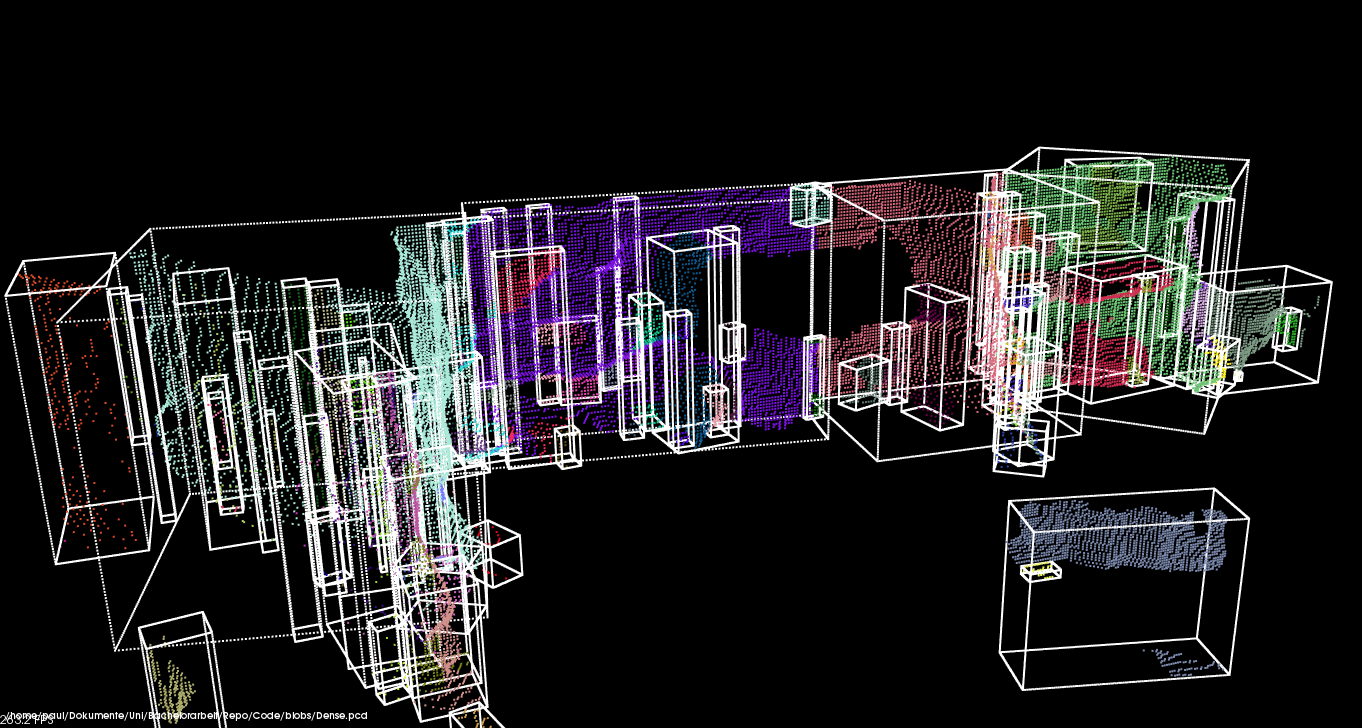
\includegraphics[width=\textwidth]{pc1OverClustering.png}
    \caption{The wall in the background is combined into many clusters}
    \label{fig:eval:pc1OverClustering}
\end{figure}

\subsubsection{Outliers} \label{sec:eval:outlier}
In the four corners of the depth-image there are a points with wrong depth estimates.
This leads to four rays consisting of these outliers in the point cloud. 
To remove these rays the point cloud gets cropped before inserting the points into the grid. 
The region of interest for cropping needs to be large enough to contain all points, even in extreme situations such as on the slope.
As a result some of these outlier points, especially close to the vehicle where they are close to the real points, are included in the region of interest.

This leads to the problem seen in Figure \ref{fig:eval:pc0Clutter}, the four small clusters in the foreground consist primarily of ground points.
But due to some outlier points below the relevant points the cells get classified as Foreground.

Due to the frequent occurrence of this problem there is sufficient training data for the \ac{cnn} which show such patches. As a result the cells with outliers get classified reliably as Clutter.
\begin{figure}[h!]
    \centering
    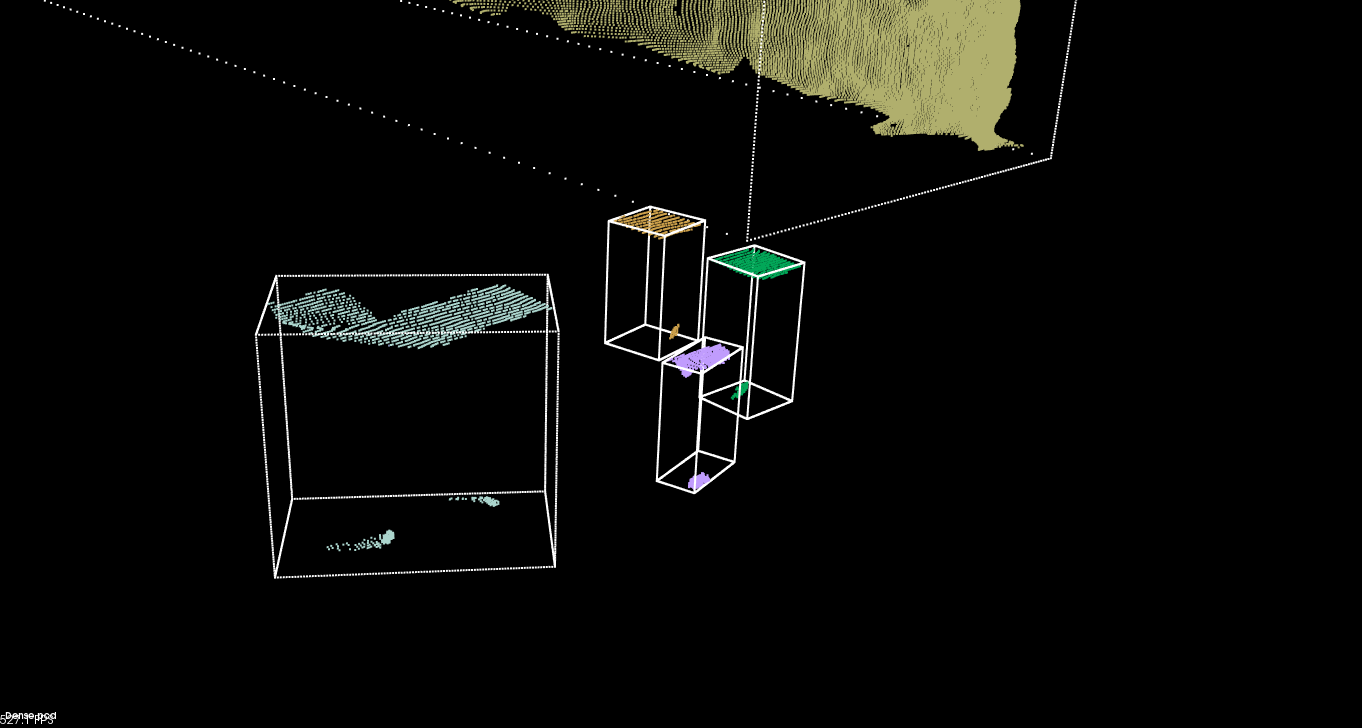
\includegraphics[width=\textwidth]{pc0Clutter.png}
    \caption{Clutter close to the vehicle}
    \label{fig:eval:pc0Clutter}
\end{figure}

\subsection{Expected Behaviour}
\subsubsection{Signs}
For obstacles and signs, such as the one shown in Figure \ref{fig:eval:pc1Sign} the bounding box is estimated correctly. 
As the bounding box is selected in such way that all points of the cluster lie within the box,
the later steps in the vehicle software, such as planning, have a good bounding box to avoid the obstacle.
Furthermore this provides a good region of interest for the classification of signs as the complete sign is visible in the extracted patch.

\begin{figure}[h!]
    \centering
    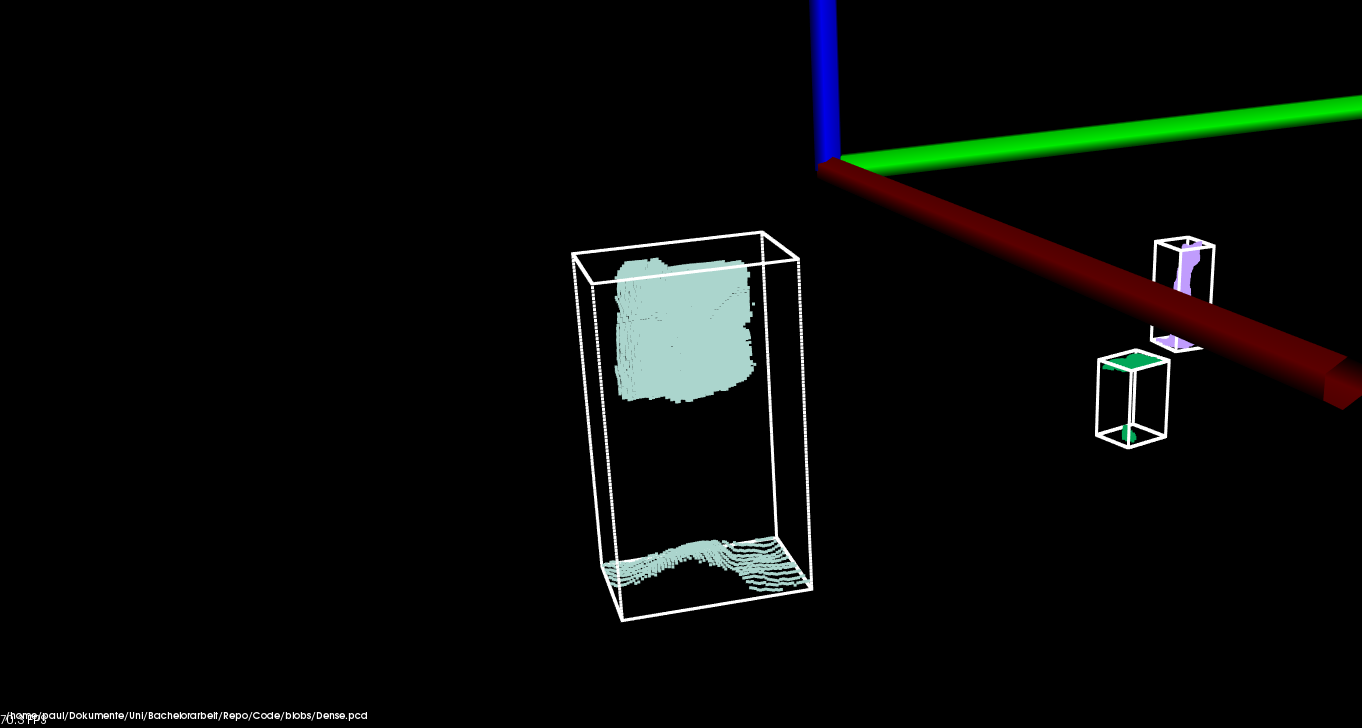
\includegraphics[width=\textwidth]{pc1Sign.png}
    \caption{Detected sign}
    \label{fig:eval:pc1Sign}
\end{figure}

\subsubsection{Obstacle touching the guardrail}
Figure \ref{fig:eval:pc0NotMerged} shows an obstacle touching the guardrail of the ramp, the guardrail is visible on the bottom left, the obstacle is in the centre of the image. 
In the point cloud there is no gap between the points which belong to the obstacle and the points which belong to the guardrail. 

In this difficult situation the separation of the two objects on subcell level is still possible due to the difference in density in both cells. As the obstacle is higher than the guardrail it contains more points and thus has a higher density. The current obstacle detection is not able to separate the objects.
\begin{figure}[h!]
    \centering
    \begin{tikzpicture}
        \node[anchor=south west,inner sep=0] at (0,0) {
            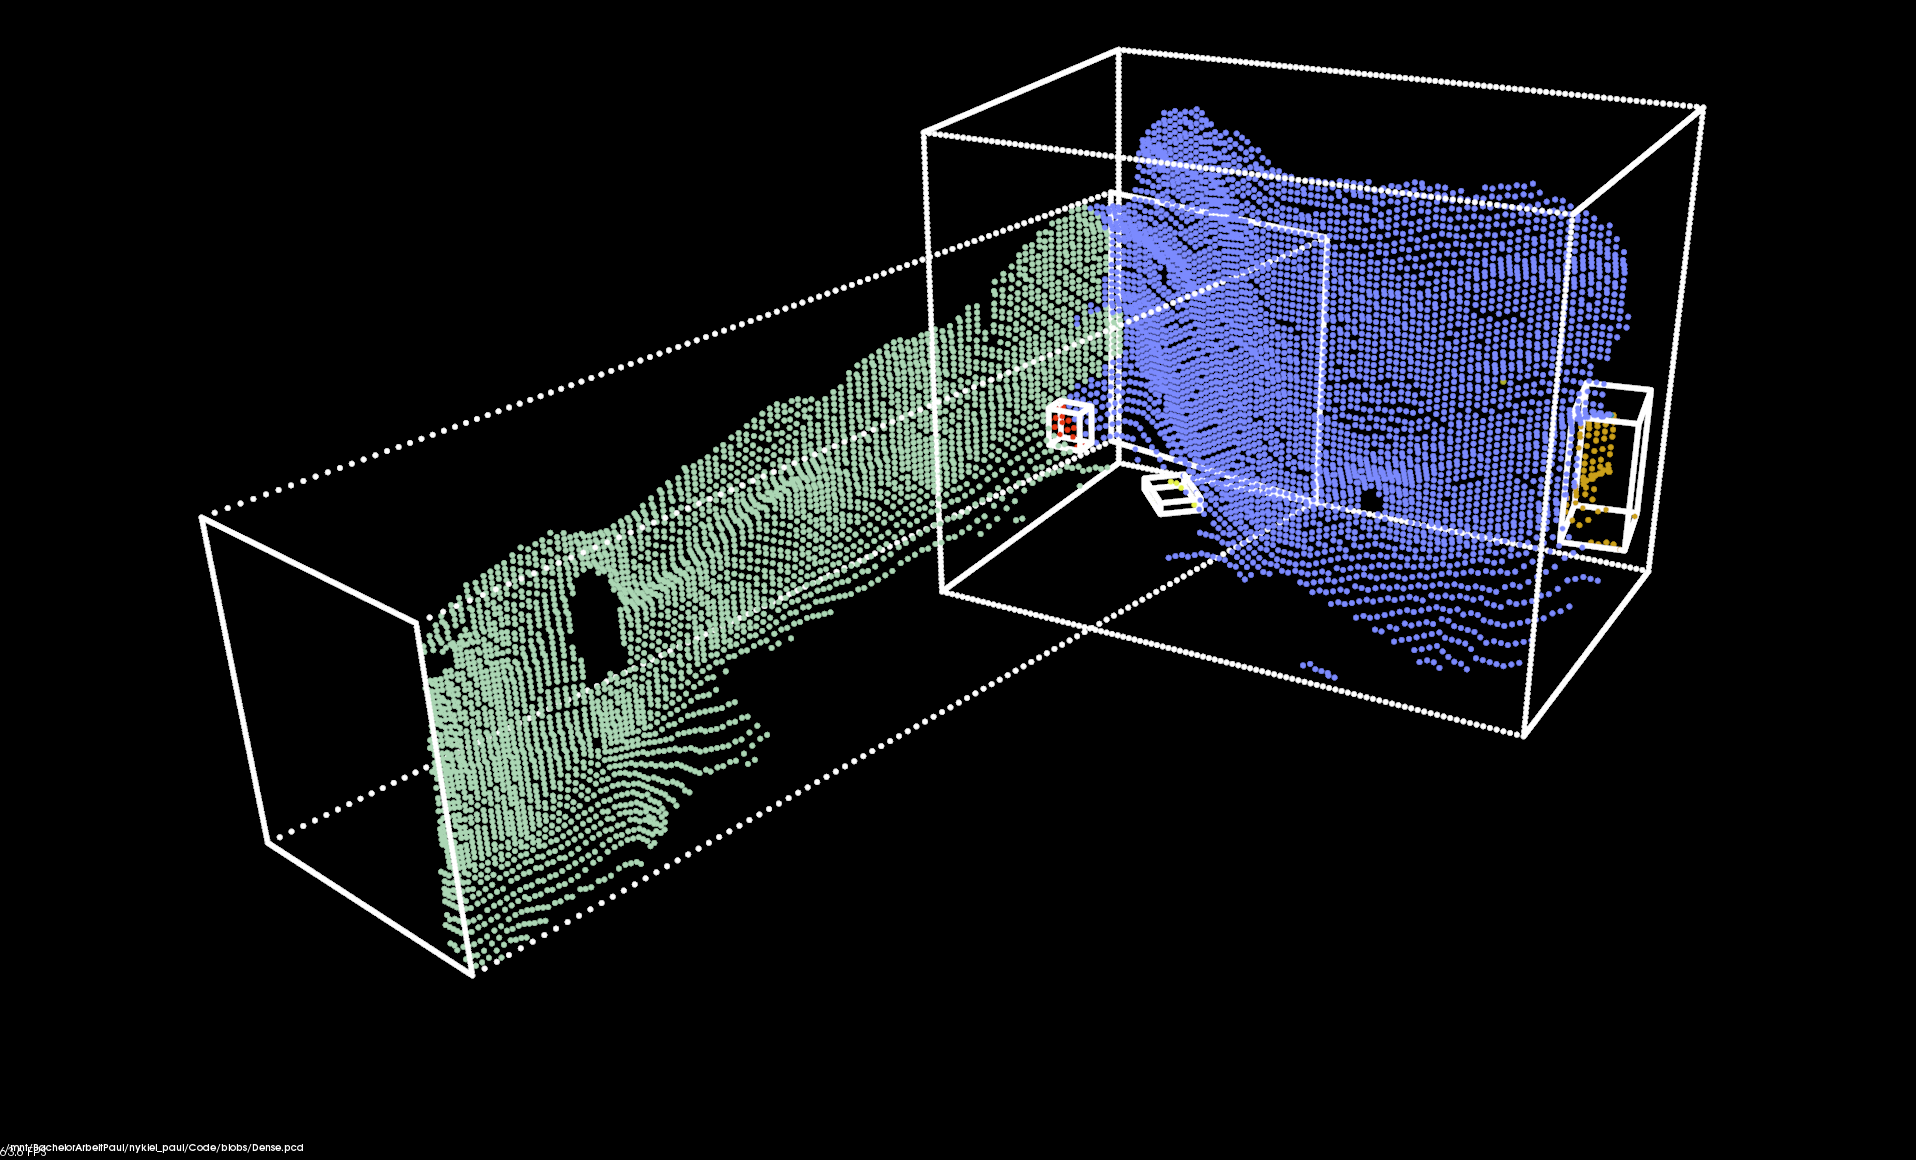
\includegraphics[width=\textwidth]{pc0NotMerged.png}
        };
        \node at (4,7) {Guardrail};
        \node at (11,9) {Obstacle};
    \end{tikzpicture}
    \caption{Obstacle close to the guardrail}
    \label{fig:eval:pc0NotMerged}
\end{figure}

\section{Computational Performance}
The \ac{d435} produces up to 30 frames per second at the maximum resolution, this limits the time for each run of the algorithm on a point cloud to 33ms.
Therefore it is required that the algorithm runs on average faster than 33ms.
In the following section the performance of the algorithm is evaluated.

\subsection{Setup}
The evaluation of the computational performance is done with a reference system similar to the system in the vehicle, as the vehicle was not available at the time of writing.
The system is equipped with an Intel\copyright Core\texttrademark i7-6700 CPU which similar in performance to the Intel\copyright Core\texttrademark i7-6770HQ CPU used in the vehicle.
The \ac{nuc} which is used in the vehicle only provides the integrated \ac{gpu}, there is no dedicated \ac{gpu}. 
Most frameworks used for neural networks, such as TensorFlow which is used here, require a Nvidia-\ac{gpu} which is able to use \ac{cuda} \cite{tensorflow2019}. As the integrated \ac{gpu} does not support \ac{cuda} it is not possible to accelerate the computations of neural networks. Therefore the \ac{gpu} in the reference system is not used for the evaluation.

Ubuntu 18.04 is used as the \ac{os}, with GCC-8 as the compiler for the software.

All steps of the algorithm are run sequentially to reduce the effects introduced by the scheduler of the \ac{os}.

\subsection{Overall Performance}
The runtime of the algorithm is measured on the 20 ground truth point clouds. 
To achieve more precise results the algorithm is run 100 times for every point cloud. 
Over all runs the mean and the standard deviation is calculated. 
Not only the overall runtime is measured but additionally the runtime for every part of the algorithm is measured.

\begin{table}[h!]
    \centering
    \begin{tabular}{l|S[table-format=2.2]S[table-format=1.3]}
        \toprule
         & {Average runtime} & {Standard deviation} \\
        \midrule
        Segmentation & 2.1ms & 0.49ms \\
        Clustering & 1.2ms & 0.52ms \\
        Extraction & 0.62ms & 0.25ms \\
        Classification & 15ms & 10ms \\
        Bounding Box Estimate & 0.73ms & 0.29ms \\
        Ground Estimate & 0.12ms & 0.046ms \\
        \midrule
        All & 19ms & 11ms \\
        \bottomrule
    \end{tabular}
    \caption{Runtime of the algorithm}
    \label{tab:eval:runtime}
\end{table}

The results can be seen in Table \ref{tab:eval:runtime}. 
Most of the time is used for the classification with the \ac{cnn}. 
The only other steps which require more than one millisecond on average is the creation of the grid and the clustering on the grid using connected components labeling on two levels. 
For the creation of the grid the most time is used for inserting all points in the grid, this is due to the large number of points. 
For the clustering the most time is used for the clustering of the fine clusters.

The average runtime is well below the time for one frame (33.3ms), this shows that the algorithm can be used on the vehicle.

\subsection{Runtime of the CNN}
As the \ac{cnn} is the part of the algorithm which requires by far the most time, its performance is evaluated in more detail.

Figure \ref{fig:eval:runtime_cnn} shows the runtime of the CNN for all patches against the number of patches. As expected the measurements are all more or less on a straight line, this shows that the runtime is proportional to the number of patches. 

\begin{figure}[h!]
    \centering
    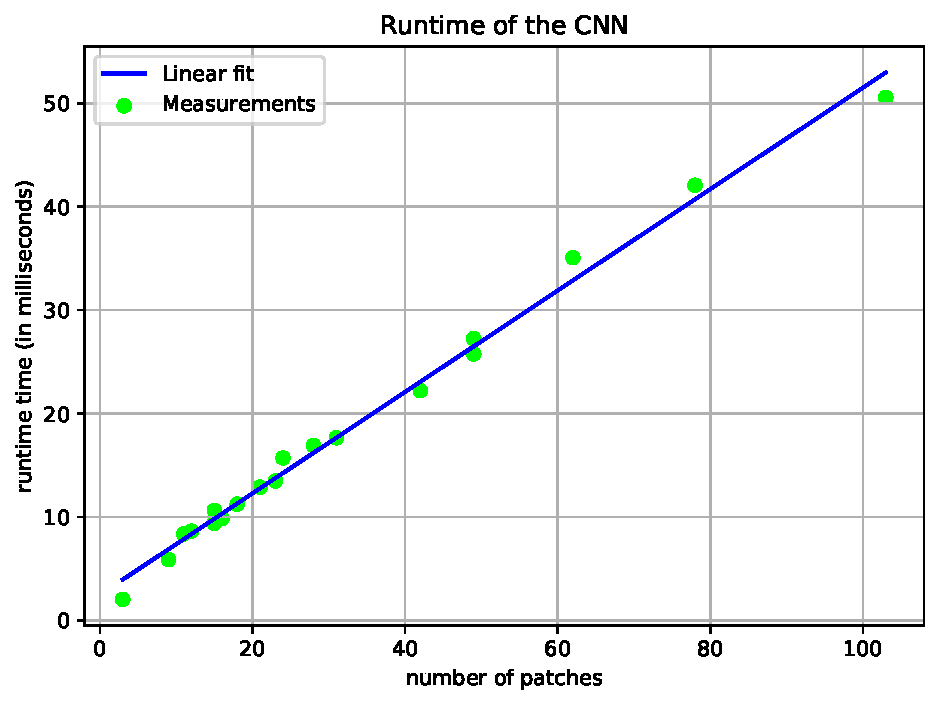
\includegraphics[width=\textwidth]{../Material/runtime_cnn.pdf}
    \caption{Plot of the runtime of the CNN against the number of patches}
    \label{fig:eval:runtime_cnn}
\end{figure}

Using least-squares regression a straight line can be fitted to the data. This line is given by:
\begin{equation}
    y = 0.49 \cdot x + 2.5
\end{equation}

The slope of the straight is 0.49 which is the average time in milliseconds per patch.

The average runtime of all steps of the algorithm but the CNN is on average 4.77ms. 
The maximum time the algorithm should require is 33ms, with these numbers the maximum number of patches which can be classified on average can be calculated:
\begin{equation}
    n_\text{max} = \frac{33 - 4.77}{0.49} = 57.6
\end{equation}

The clusters get extracted from the grid from near to far, the classification is started with objects which are closer to the vehicle. 
These objects are of greater importance, as these are the objects the vehicle has to handle first.

If the algorithm is required to finish in the given 33ms the classification can be stopped after a certain time. 
On average it is possible to classify 57 patches in this time frame. 
Compared to the relatively low number of relevant objects close to the vehicle this suffices to detect all relevant objects.

\section{Evaluation on real world data}
According to \cite{Wang19} object detection on stereo data can be vastly improved by representing the data as a point cloud instead of a disparity map. 
To verify this the algorithm should not only run on the data from the \ac{d435} but additionally on real world data.

The point clouds used as an input for the algorithm are calculated from two colour images. For the calculation of the disparity map semi-global block matching, an improved version of semi-global matching (see \ref{sec:theo:sgm}) is used.
From the disparity map the point cloud is calculated, as explained in \ref{sec:theor:disp2pc}.
In comparison to the data provided by the \ac{d435} no active stereo is used, the two cameras are the only source of depth information.

\subsection{Kitti}
The baseline of the camera system is only $0.54\si{\m}$ \cite{Menze2015CVPR}, as shown in \ref{sec:theo:error} the baseline distance is inverse proportional to the depth error.
As a result the quality of the point cloud is much lower than the quality of the point clouds acquired with the \ac{d435}. 
Figure \ref{fig:eval:kittiBadImage} shows a part of one of the two images used for the stereo extraction. 
The image is part of the Kitti dataset \cite{Menze2015CVPR}. 
Figure \ref{fig:eval:kittiBad} shows a part of the point cloud calculated from the stereo pair.

The scene shows two cars on the opposite side of the road. 
The car that is closer, marked in red, is about 13 meters from the camera. 
Even at this distance the point cloud does not show a single blob but multiple blobs around the actual position of the vehicle.

% Testing / 005 bzw. 2_11
\begin{figure}[h!]
    \centering
    \begin{tikzpicture}
        \node[anchor=south west,inner sep=0] at (0,0) {
            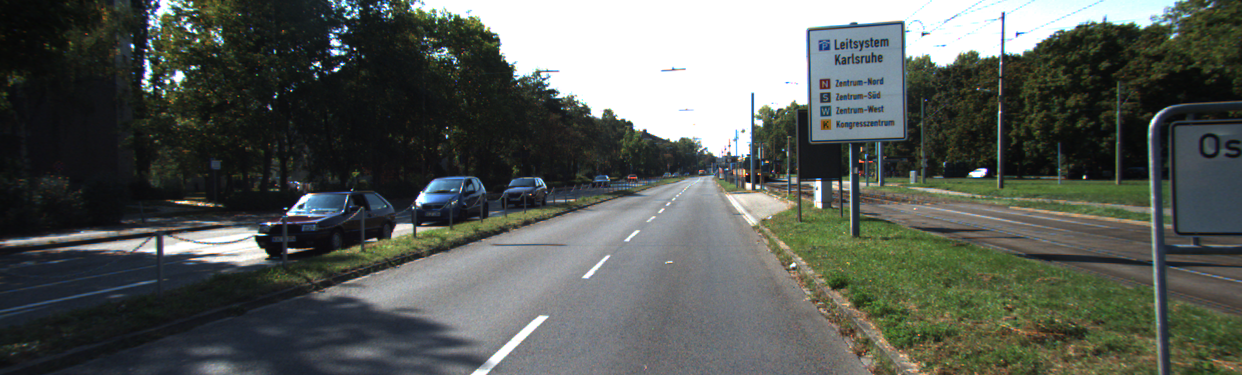
\includegraphics[width=\textwidth,trim={6cm 2cm 22cm 5cm},clip]{../Material/kittiBadImage.png}
        };
        \draw[red,ultra thick,rounded corners] (2.8,2) rectangle (7.7,4.5);
        \draw[green,ultra thick,rounded corners] (8.2,3) rectangle (10.8,5);
    \end{tikzpicture}
    \caption{Image from the Kitti dataset}
    \label{fig:eval:kittiBadImage}
\end{figure}

\begin{figure}[h!]
    \centering
    \begin{tikzpicture}
        \node[anchor=south west,inner sep=0] at (0,0) {
            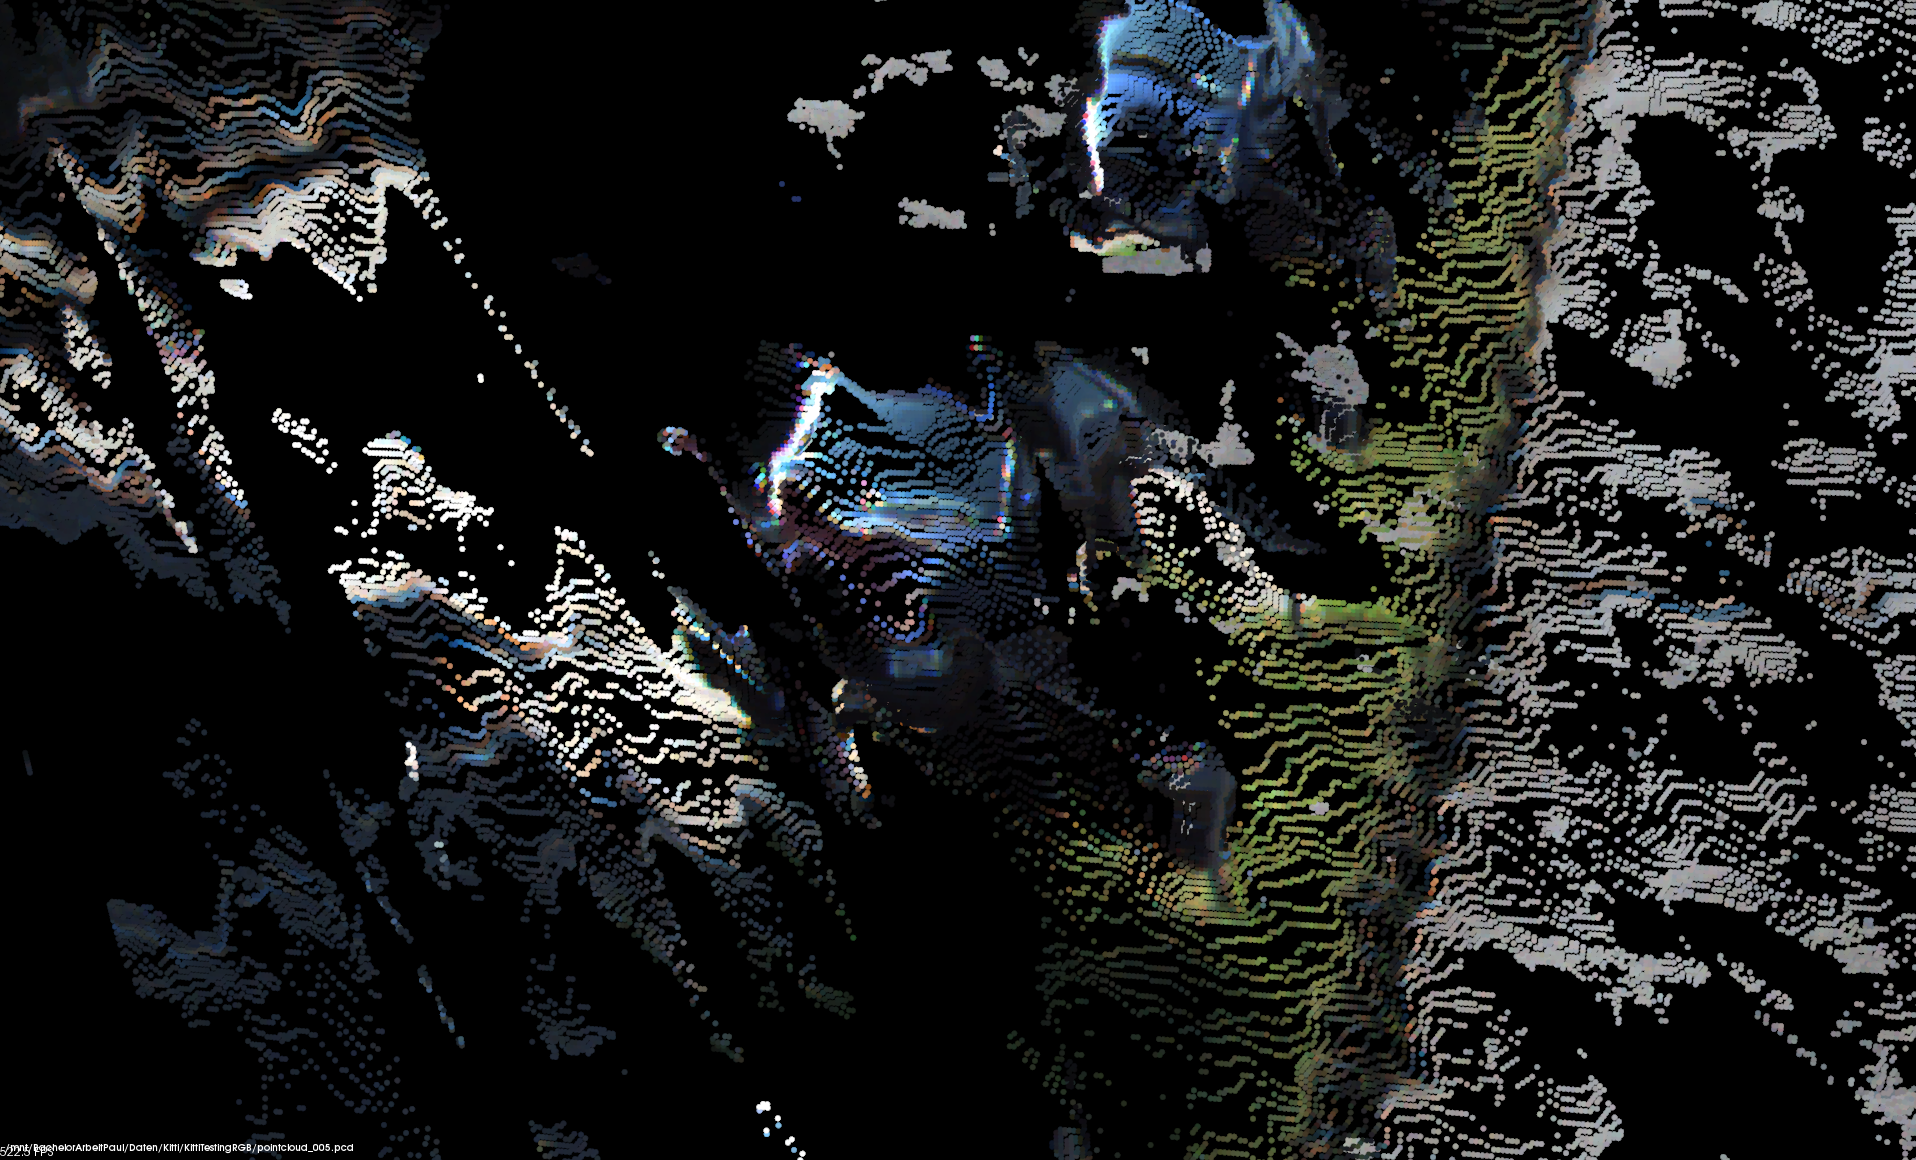
\includegraphics[width=\textwidth]{../Material/kittiBad.png}
        };
        \draw[red,ultra thick,rounded corners] (6,3.6) rectangle (9,6.6);
        \draw[green,ultra thick,rounded corners] (8.3,7.2) rectangle (10.5,9.2);
    \end{tikzpicture}
    \caption{Bird's-eye view of two vehicles in a point cloud generated from Kitti data}
    \label{fig:eval:kittiBad}
\end{figure}

The poor quality of the point cloud results in many small clusters due to the large variance in density throughout a single object. Therefore the patches that get extracted from the point cloud seldomly show the complete object, most of the time only parts of the objects are shown, subsequently the \ac{cnn} yields a poor performance.

To increase the accuracy of the classification the colour information of the point cloud is used to generate patches, which show the relevant object. Figure \ref{fig:eval:texture} shows examples for such patches.
The first row (Figures \ref{fig:eval:texture:222_0}, \ref{fig:eval:texture:222_0} and \ref{fig:eval:texture:0_0}) show all objects which are closer than 10 meters to the cameras.
The second row (Figures \ref{fig:eval:texture:0_1} and \ref{fig:eval:texture:0_1}) show objects at a larger distance.
For the objects closer than 10 meters the algorithm is able to correctly detect the objects and extract patches which show the complete vehicle. 
At a larger distance a single object in the point cloud is split up into multiple objects by the detection.
Therefore multiple patches which show only a part of the vehicle are extracted.

\begin{figure}[h!]
    \centering
    \begin{subfigure}[c]{0.3\textwidth}
        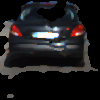
\includegraphics[width=\textwidth]{../Material/texture222_0.png}
        \subcaption{Car}
        \label{fig:eval:texture:222_0}
    \end{subfigure}
    \begin{subfigure}[c]{0.3\textwidth}
        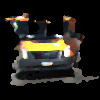
\includegraphics[width=\textwidth]{../Material/texture222_1.png}
        \subcaption{Van}
        \label{fig:eval:texture:222_1}
    \end{subfigure}
    \begin{subfigure}[c]{0.3\textwidth}
        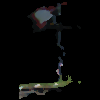
\includegraphics[width=\textwidth]{../Material/texture0_0.png}
        \subcaption{Sign}
        \label{fig:eval:texture:0_0}
    \end{subfigure}
    \begin{subfigure}[c]{0.3\textwidth}
        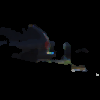
\includegraphics[width=\textwidth]{../Material/texture0_1.png}
        \subcaption{Rear of a car}
        \label{fig:eval:texture:0_1}
    \end{subfigure}
    \begin{subfigure}[c]{0.3\textwidth}
        
\includegraphics[width=\textwidth]{../Material/texture0_2.png}
        \subcaption{Centre of a car}
        \label{fig:eval:texture:0_2}
    \end{subfigure}
    \caption{Patches extracted from Kitti data}
    \label{fig:eval:texture}
\end{figure}

\subsection{Ulm-Lehr}
For the data acquired by the pilot installation in Ulm-Lehr the quality of the point cloud is better due to the larger distance of the cameras.
As the cameras are stationary they all show the same scene. The scene depicts a flat road with vehicles, no slopes are present. 
Due to the elevated mounting position of the camera system most parts of the road are visible at all times. 
In contrast objects in the Kitti dataset are often occluded by other objects.

The evaluation is done using the \ac{iou}, similar to section \ref{sec:eval:iou}. For the evaluation 2,322 labeled point clouds with 4,725 objects in total are used.
Out of the 4,725 objects 4,171 objects are detected by the algorithm, this is a detection rate of 88\%. 
Figure \ref{fig:eval:iouDistLehr} shows the histograms of the two- and three-dimensional \ac{iou}-scores, the average two dimensional \ac{iou}-score is 0.53, the average three-dimensional-score 0.43.

\begin{figure}[h!]
    \centering
    \begin{subfigure}[c]{0.48\textwidth}
        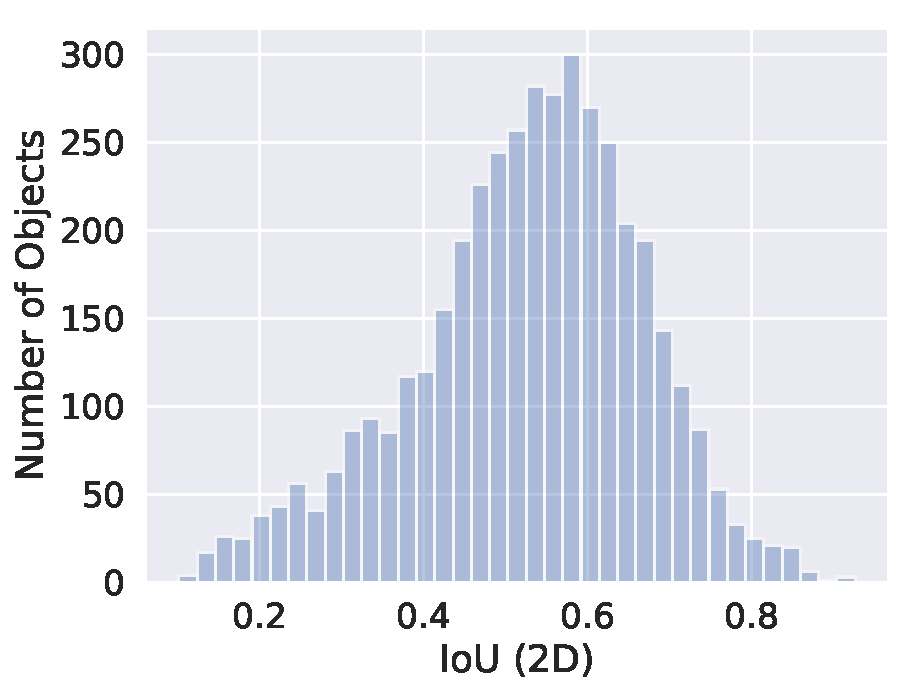
\includegraphics[width=\textwidth]{../Material/iou2_lehr.pdf}
        \subcaption{2D}
    \end{subfigure}
    \begin{subfigure}[c]{0.48\textwidth}
        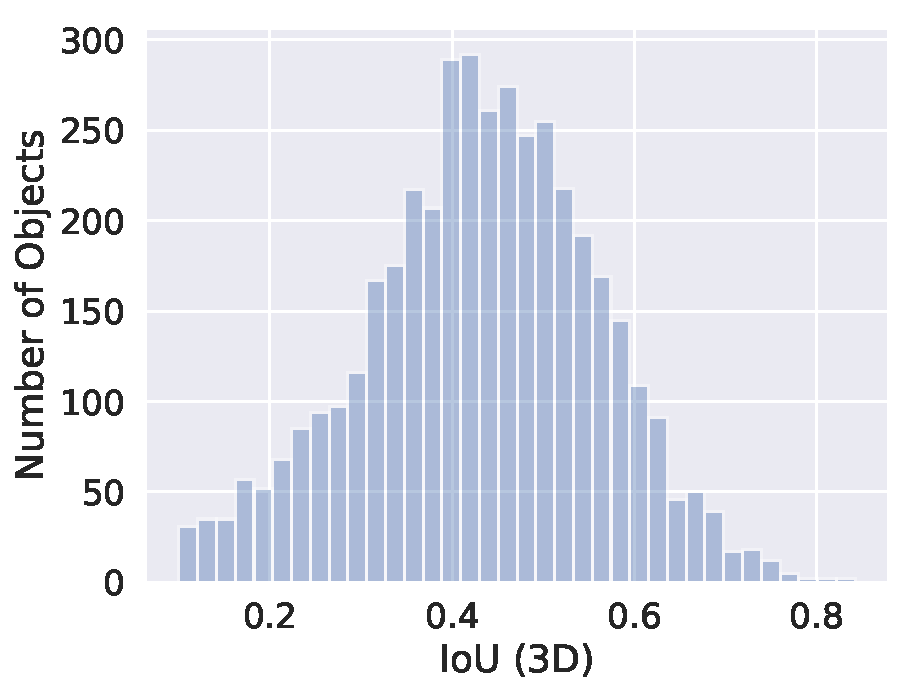
\includegraphics[width=\textwidth]{../Material/iou3_lehr.pdf}
        \subcaption{3D}
    \end{subfigure}
    \caption{Distribution of the IoU-Scores}
    \label{fig:eval:iouDistLehr}
\end{figure}

Both \ac{iou}-scores are higher than the respective score for the \ac{d435} data. This is primarily due to the simplicity of the scene and the elevated camera position.

Figure \ref{fig:eval:iouLehr} shows examples of the detections and the corresponding ground truth data. Objects closer than 50 meters, such as the ones shown in Figure \ref{fig:eval:iouLehr:2} generate an accurate bounding box. At distances over 50 meters, some objects can still be detected, like the object seen in \ref{fig:eval:iouLehr:1} but there is some noise present.

\begin{figure}[h!]
    \centering
    \begin{subfigure}[c]{0.75\textwidth}
        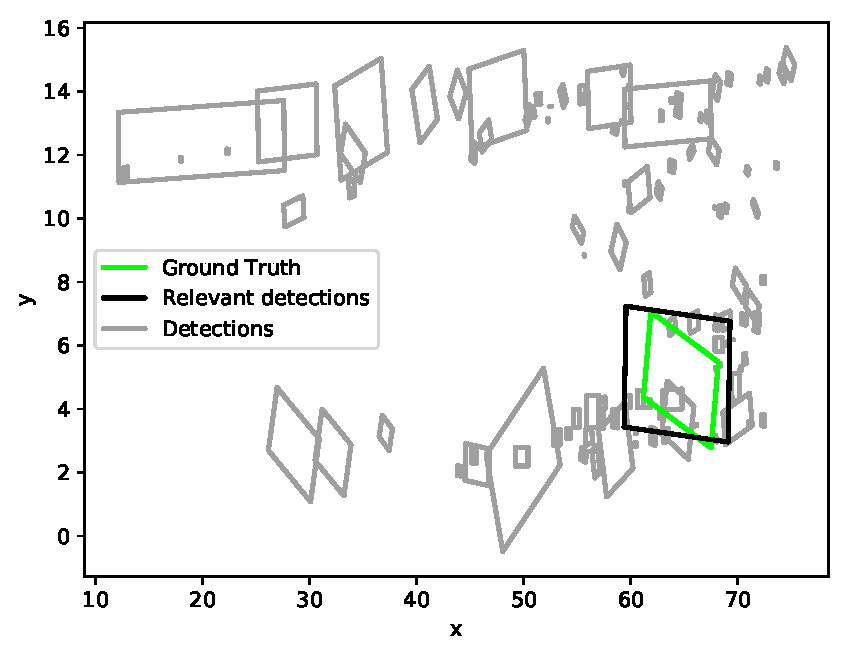
\includegraphics[width=\textwidth]{../Material/lehr1.pdf}
        \subcaption{}
        \label{fig:eval:iouLehr:1}
    \end{subfigure}
    \begin{subfigure}[c]{0.75\textwidth}
        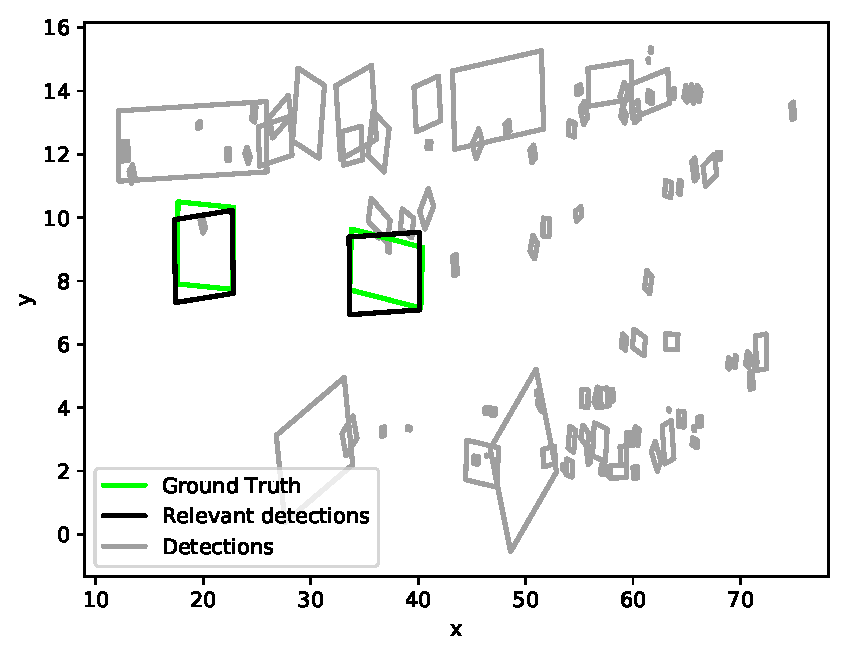
\includegraphics[width=\textwidth]{../Material/lehr2.pdf}
        \subcaption{}
        \label{fig:eval:iouLehr:2}
    \end{subfigure}
    \caption{Comparison of the estimated bounding boxes and the ground truth data, seen from above}
    \label{fig:eval:iouLehr}
\end{figure}

\section{Comparison with other algorithms}
Most of the current state of the art algorithms for object detection, such as \cite{shi2019}, 
\cite{Bin19} and \cite{Mar18}, use deep neural networks for detection and classification of the objects.
The large \ac{cnn}s used for this end-to-end detection require a lot of computational power.
\cite{Mar18} states, that Complex-YOLO runs at 50 \ac{fps} on a NVIDIA TitanX \ac{gpu}. 
As there is no official implementation publicly available, the runtime can not be measured on the vehicle.
To estimate the performance YOLO \cite{yolov3} is used, this \ac{cnn} is used for object detection on images and is the base for Complex-YOLO.
YOLO is publicly available and runs at 30 \ac{fps} on the TitanX \ac{gpu}.

Using the numbers given in Table \ref{tab:eval:yoloRuntime} the runtime of Complex-YOLO on the vehicle can be estimated, assuming that the ratio between YOLO and Complex-YOLO is independent of the device used:
\begin{equation}
    t_\text{Complex-YOLO Vehicle} \approx \frac{t_\text{Complex-YOLO TitanX}}{t_\text{YOLO TitanX}} \cdot t_\text{YOLO Vehicle} = 31s
\end{equation}

\begin{table}[h!]
    \centering
    \begin{tabular}{c|cc}
        \toprule
         & Titan X & On the vehicle\\
         \midrule
         YOLO & 33ms & 46s \\
         Complex-YOLO & 20ms & \text{approx} 31s \\ 
         \bottomrule
    \end{tabular}
    \caption{Comparison of the runtimes (Complex-YOLO on the vehicle is estimated)}
    \label{tab:eval:yoloRuntime}
\end{table}

This is only a rough approximate but the estimated time is about three magnitudes larger than the maximum time allowed. This shows that it is not possible to use a deep neural network for end-to-end detection on the vehicle without a \ac{gpu} or dedicated hardware for acceleration of the calculations.

    \section{Fazit}
\begin{frame}
    \frametitle{Fazit}
    \begin{itemize}
        \item Algorithmus adaptiert und erweitert für Stereo Daten
            \pause
        \item Verbesserungen für Stereo Daten
            \pause
        \item Verbesserungen gegenüber aktueller Hinderniserkennung
            \pause
        \item Ergebnisse auf Echtweltdaten abhängig von Punktwolke
    \end{itemize}
\end{frame}

\begin{frame}
    \frametitle{Mögliche Verbesserungen}
    \begin{itemize}
        \item Besseres Stereo Matching
            \pause
        \item Segmentierung durch MLP
            \pause
        \item Klassifikation immer über Farbbild
    \end{itemize}
\end{frame}

\begin{frame}
    \frametitle{Abkürzungen}
    \begin{acronym}[]
    \acro{adtf}[ADTF]{Automotive Data and Time-Triggered Framework}
    \acro{cnn}[CNN]{Convolutional Neural Network}
    \acro{cuda}[CUDA]{Compute Unified Device Architecture}
    \acro{d435}[D435]{Intel\textsuperscript{\textcopyright{}} RealSense\texttrademark{} Depth Camera D435}
    \acro{fps}[FPS]{Frames per second}
    \acro{gpu}[GPU]{Graphics processing unit}
    \acro{iou}[IoU]{Intersection over Union}
    \acro{mlp}[MLP]{Multilayer Perceptron}
    \acro{mse}[MSE]{Mean Square Error}
    \acro{nuc}[NUC]{Next Unit of Computing}
    \acro{os}[OS]{Operating system}
    \acro{pca}[PCA]{Principal Component Analysis}
    \acro{rc}[RC]{Radio Controlled}
    \acro{relu}[ReLU]{Rectified Linear Unit}
    \acro{sgd}[SGD]{Stochastic Gradient Descent}
\end{acronym}

\end{frame}

    \section*{}
\begin{frame}
    \frametitle{Abschätzung Laufzeit}
    \begin{tabular}{c|cc}
        \toprule
         & Titan X & Fahrzeug \\
         \midrule
         YOLO & 33ms & 46s \\
         Complex-YOLO & 20ms & \text{ca.} 31s \\ 
         \bottomrule
    \end{tabular}
\end{frame}

\begin{frame}
    \frametitle{CNN}
    \hspace*{-1cm}
    \begin{tikzpicture}[scale=0.58]
        \node[anchor=south west,inner sep=0] at (0,0) {
            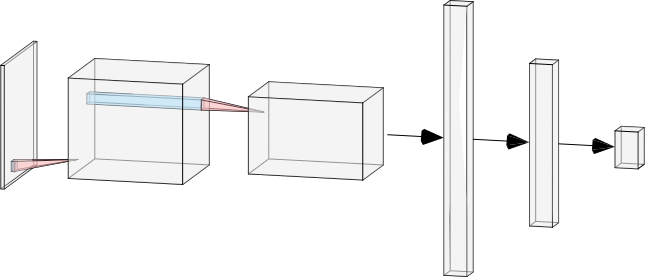
\includegraphics[width=.9\textwidth]{cnn.pdf}
        };

        \node at (1,-0.5) {Convolution};
        \node at (5,-0.5) {Convolution};
        \node at (9.5,-0.5) {Flatten};
        \node at (11.8,-0.5) {Dense};
        \node at (14,-0.5) {Dense};

        \node at (0.3,7) {$40\times40\times1$};
        \node at (3.3,6) {$20\times20\times32$};
        \node at (7.4,7) {$10\times10\times32$};
        \node at (10.8,7) {$3200$};
        \node at (12.8,7) {$128$};
        \node at (14.9,7) {$3$};
    \end{tikzpicture}
\end{frame}

\begin{frame}
    \frametitle{Segmentierung - Punktweise}
    \setlength{\tabcolsep}{1pt}
    \hspace*{-1.8cm}
    \begin{tabular}{c|rrrrrr}
        \toprule
        \diagbox{Predicted}{Actual} & \multicolumn{2}{c}{Ground} & \multicolumn{2}{c}{Foreground} & \multicolumn{2}{c}{Sparse} \\
        \midrule
        Ground & 958,704 & (92.1\%) & 3,436 & (2.0\%) & 12,224 & (53.3\%) \\ 
        Foreground & 70,293 & (6.8\%) & 164,209 & (97.9\%) & 10,416 & (45.4\%)  \\ 
        Sparse & 11,688 & (1.1\%) & 71 & (0.04\%) & 273 & (1.2\%) \\ 
        \midrule
        Gesamt & 1,040,685 && 167,716 && 22,913 \\
        \bottomrule
    \end{tabular}
\end{frame}

\begin{frame}
    \frametitle{Segmentierung - Zellenweise}
    \setlength{\tabcolsep}{3pt}
    \hspace*{-1.6cm}
    \begin{tabular}{c|rrrrrr}
        \toprule
        \diagbox{Predicted}{Actual} & \multicolumn{2}{c}{Ground} & \multicolumn{2}{c}{Foreground} & \multicolumn{2}{c}{Sparse} \\
        \midrule
        Ground & 8,302 & (96.9\%) & 45 & (14.8\%) & 227 & (0.45\%) \\
        Foreground & 184 & (2.1\%) & 248 & (81\%) & 45 & (0.1\%) \\
        Sparse & 79 & (0.92\%) & 12 & (4.0\%) & 49,943 & (99.5\%) \\
        \midrule
        Gesamt & 8,565 && 305 && 50,215 \\
        \bottomrule
    \end{tabular}
\end{frame}

\begin{frame}
    \frametitle{Clustering und Bounding-Box Schätzung}
    \begin{columns}
        \begin{column}{.5\textwidth}
            \begin{tabular}{cc}
                \toprule
                Durchschnitt 2D & 0.444 \\
                Durchschnitt 3D & 0.321 \\
                \bottomrule
            \end{tabular}
        \end{column}
        \begin{column}{.5\textwidth}
            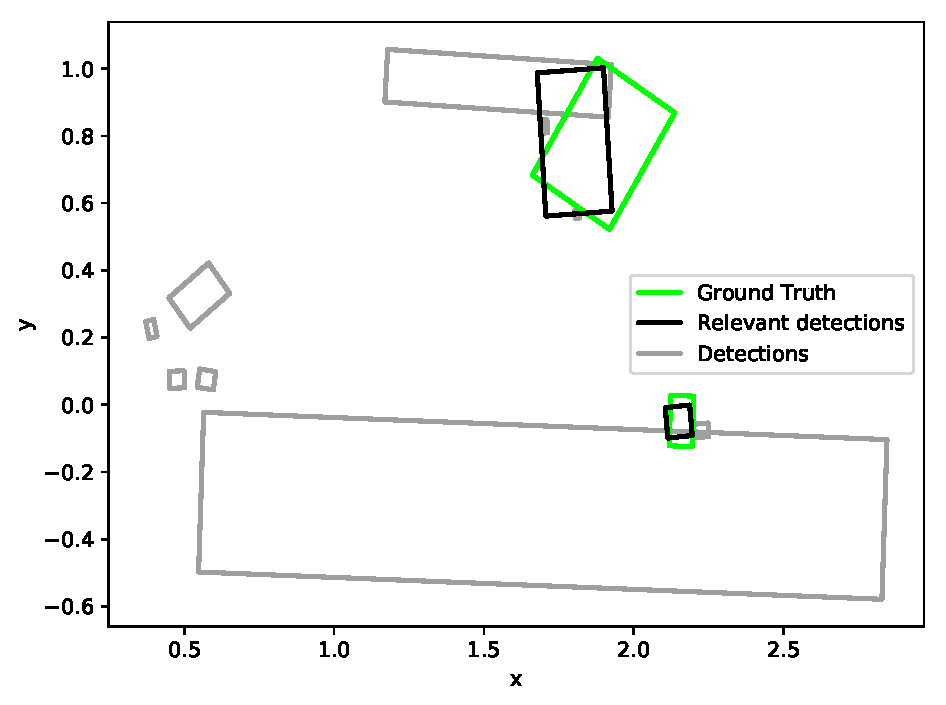
\includegraphics[width=\textwidth]{../Material/iou0.pdf}
            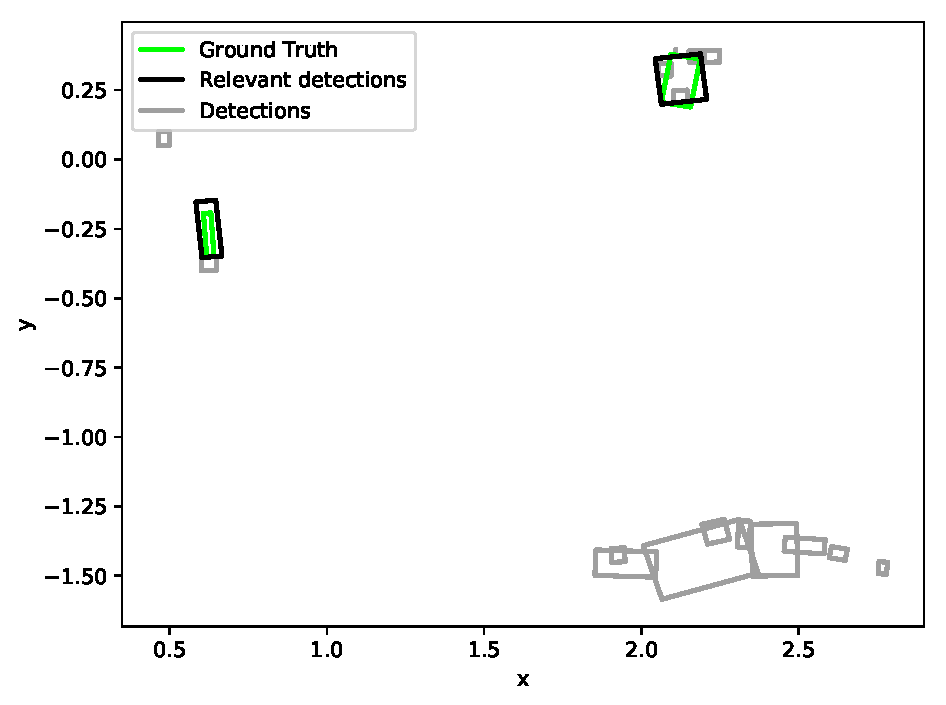
\includegraphics[width=\textwidth]{../Material/iou2.pdf}
        \end{column}
    \end{columns}
\end{frame}

\begin{frame}
    \frametitle{Klassifikation}
    \setlength{\tabcolsep}{3pt}
    \hspace*{-1.0cm}
    \begin{tabular}{c|rrrrrr}
        \toprule
        \diagbox{Predicted}{Actual} & \multicolumn{2}{c}{Clutter} & \multicolumn{2}{c}{Obstacle} & \multicolumn{2}{c}{Sign} \\
        \midrule
        Clutter & 555 & (89.5\%) & 3 & (15.8\%) & 3 & (16.7\%) \\
        Obstacle & 49 & (7.9\%) & 15 & (78.9\%) & 1 & (5.6\%) \\
        Sign & 16 & (2.5\%) & 1 & (5.2\%) & 14 & (77.8\%) \\
        \midrule
        Gesamt & 620 && 19 && 18 \\
        \bottomrule
    \end{tabular}
\end{frame}

\begin{frame}
    \frametitle{Evaluation - Verbesserungen}
    \hspace*{-0.5cm}
    Vorgeschlagen:

    \hspace*{-0.5cm}
    \begin{tabular}{c|c|rrr}
        \toprule
        Kategorie & Anzahl & Pr & Rc & $F_1$\\
        \midrule
        Obstacle/Pedestrian & 20 & 100\% & 84\% & 91\% \\
        Sign & 18 & 78\% & 100\% & 88\% \\
        \midrule
        Durchschnitt/Summe & 38 & 89\% & 92\% & 90\% \\
        \bottomrule
    \end{tabular}

    \vspace{0.5cm}
    \hspace*{-0.5cm}
    \cite{AttBen17}:

    \hspace*{-0.5cm}
    \begin{tabular}{c|c|rrr}
        \toprule
        Kategorie & Anzahl & Pr & Rc & $F_1$\\
        \midrule
        Obstacle/Pedestrian & 20 & 100\% & 80\% & 89\% \\
        Sign & 17 & 71\% & 100\% & 83\% \\
        \midrule
        Durchschnitt/Summe& 37 & 86\% & 90\% & 86\% \\
        \bottomrule
    \end{tabular}
\end{frame}

\begin{frame}
    \frametitle{Bodenschätzung}
    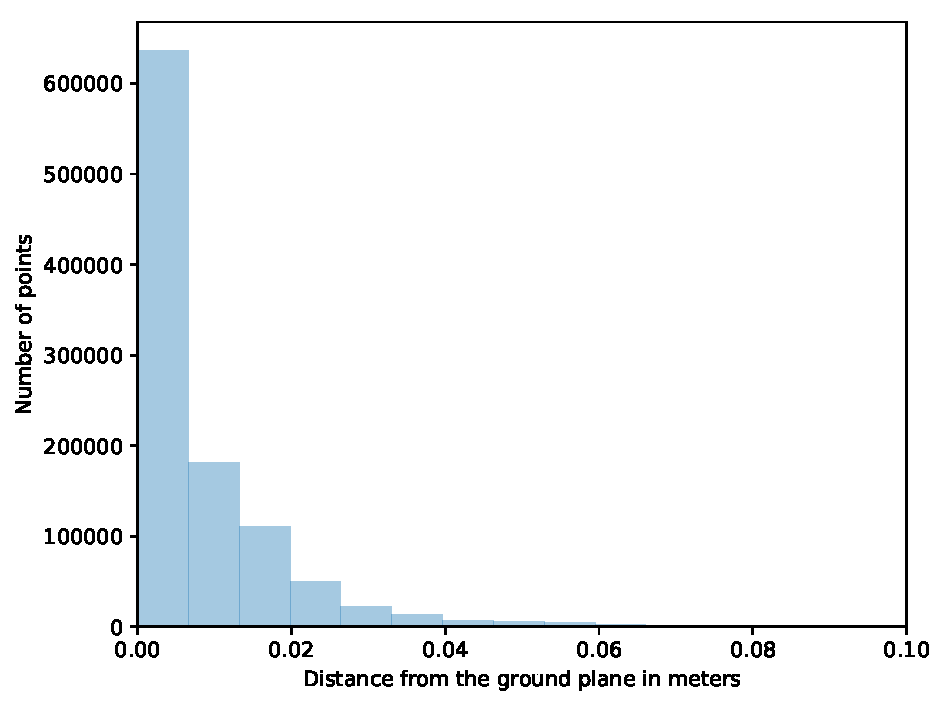
\includegraphics[width=\textwidth]{../Material/ground.pdf}
\end{frame}

\begin{frame}
    \frametitle{Evaluation Lehr}
    \begin{columns}
        \begin{column}{.5\textwidth}
            \begin{tabular}{cc}
                \toprule
                Durchschnitt 2D & 0.53\\
                Durchschnitt 3D & 0.43 \\
                \bottomrule
            \end{tabular}
        \end{column}
        \begin{column}{.5\textwidth}
            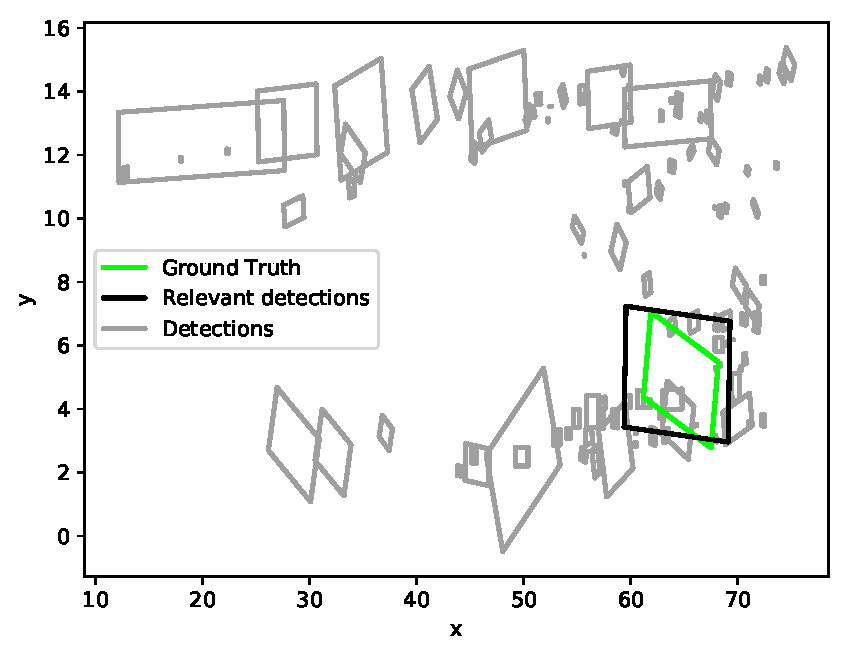
\includegraphics[width=\textwidth]{../Material/lehr1.pdf}
            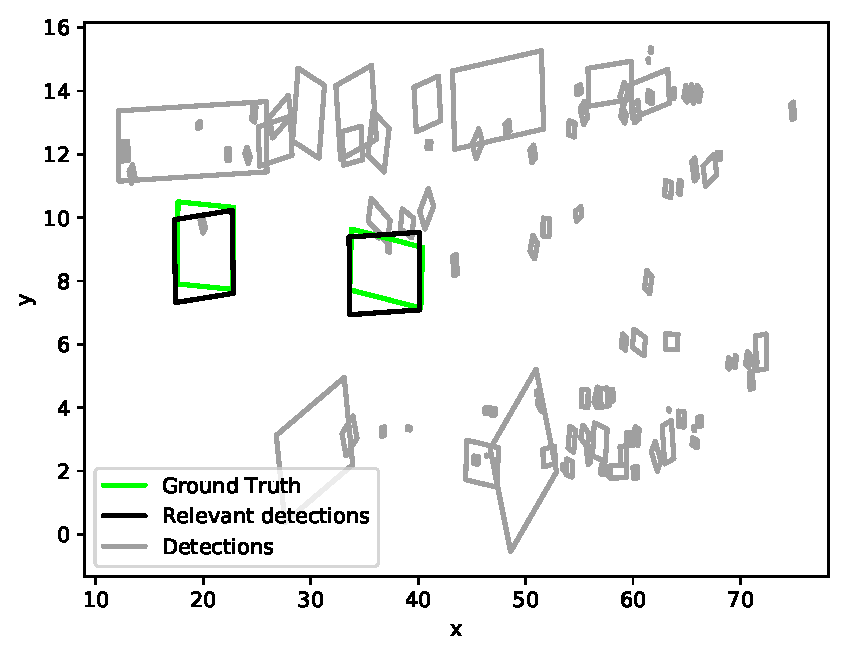
\includegraphics[width=\textwidth]{../Material/lehr2.pdf}
        \end{column}
    \end{columns}
\end{frame}

\end{document}
